% % \section{Использованные функции}

% % \begin{lstlisting}[caption={Функция для отображения исходного и преобразованного изображений}]
% % # show the source image and transformed image
% % def show_images(source, transformed, title="Image"):
% %     img_src_rgb = cv2.cvtColor(source, cv2.COLOR_BGR2RGB) # normal colors to display
% %     img_trf_rgb = cv2.cvtColor(transformed, cv2.COLOR_BGR2RGB) 

% %     plt.figure(figsize=(13, 5))
% %     plt.suptitle(title, fontsize=16)

% %     plt.subplot(1, 2, 1)
% %     plt.imshow(img_src_rgb)
% %     plt.title('Source Image')
% %     plt.text(10, 10, f'Resolution: {source.shape[1]}x{source.shape[0]}', color='white', backgroundcolor='black', fontsize=8, ha='left', va='top')
% %     plt.axis('off')

% %     plt.subplot(1, 2, 2)
% %     plt.imshow(img_trf_rgb)
% %     plt.title('Transformed Image')
% %     plt.text(10, 10, f'Resolution: {transformed.shape[1]}x{transformed.shape[0]}', color='white', backgroundcolor='black', fontsize=8, ha='left', va='top')
% %     plt.axis('off')

% %     # adjust space between images
% %     plt.subplots_adjust(wspace=0.3, hspace=0.3)
% %     plt.subplots_adjust(left=0.05, right=0.95)

% %     # save image
% %     plt.savefig(f"results/{title}.png")
% % \end{lstlisting}

% % \begin{lstlisting}[caption={Функция для применения матричных преобразований}]
% % def apply_matrix_transformations(img, matrix, shape=(0, 0)):
% %     # apply the matrix to the image
% %     if shape == (0, 0):
% %         shape = (img.shape[1], img.shape[0])
% %     return cv2.warpAffine(img, matrix, shape)
% % \end{lstlisting}

% % \begin{lstlisting}[caption={Функция для применения проективных преобразований}]
% % def apply_perspective_transformations(img, matrix, shape=(0, 0)):
% %     # apply the matrix to the image
% %     if shape == (0, 0):
% %         shape = (img.shape[1], img.shape[0])
% %     return cv2.warpPerspective(img, matrix, shape)
% % \end{lstlisting}

% % \begin{lstlisting}[caption={Функция для коррекции дисторсии}]
% % def distortion_correction(img, map_func):
% %     xi, yi = np.meshgrid(np.arange(img.shape[1]), np.arange(img.shape[0]))

% %     # shift and normalize grid 
% %     xmid, xmid = img.shape[1] / 2.0, img.shape[0] / 2.0
% %     xi = xi - xmid
% %     yi = yi - xmid

% %     # convert to polar coordinates
% %     r, theta = cv2.cartToPolar(xi / xmid, yi / xmid)
% %     r = map_func(r)

% %     # convert back to cartesian coordinates
% %     u, v = cv2.polarToCart(r, theta)

% %     u, v = u * xmid + xmid, v * xmid + xmid

% %     # remap the image
% %     return cv2.remap(img, u.astype(np.float32), v.astype(np.float32), cv2.INTER_LINEAR)
% % \end{lstlisting}

\href{https://github.com/mfclabber/itmo-cv-labs/tree/main/lab3}{Исходный код на GitHub}. 

\section{Теоретическая часть}

Цифровые изображения, полученные различными оптико-электронными приборами, 
могут содержать в себе разнообразныеискажения, обусловленные разного рода помехами, 
которые принято называть шумом. Шум на изображении затрудняет его обработку
автоматическими средствами, и, поскольку шум может иметь различную природу, 
для его успешного подавления необходимо определить адекватную математическую модель.

Для удобства отладки и сборки используется средство автоматизации сборки ПО CMake:
\begin{lstlisting}[style=cpp_white, caption={CMakeLists.txt для сборки проекта}]
cmake_minimum_required(VERSION 2.8)

project( CV_LW3 )
find_package( OpenCV REQUIRED )

include_directories( ${OpenCV_INCLUDE_DIRS} )
add_executable( ${PROJECT_NAME}  src/lab2.cpp )

target_link_libraries( ${PROJECT_NAME} ${OpenCV_LIBS} )
\end{lstlisting}

\pagebreak

Возьмем одно изображение из датасета беспилотников Яндекса и наложим на него различные шумы
\begin{figure}[ht]
    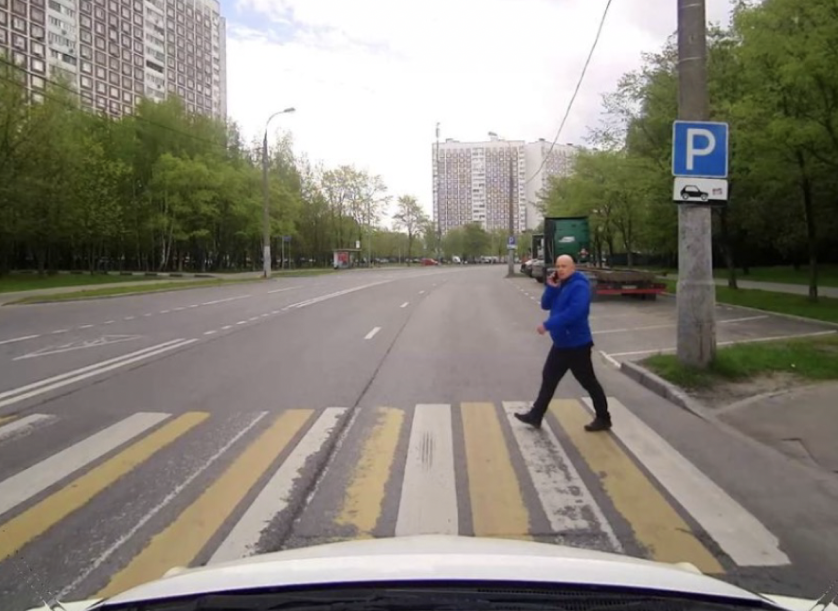
\includegraphics[width=\textwidth]{../source/image.png}
    \caption{Исходное изображение}
    \label{fig:source_image}
\end{figure}


\section{Типы шумов}

\subsection{Импульсный шум}

При импульсном шуме сигнал искажается выбросами с очень
большими отрицательными или положительными значениями малой длительностью и может возникать,например, из-за ошибок
декодирования. Такой шум приводит к появлению на изображении белых («соль») или черных («перец») точек, поэтому зачастую
называется точечным шумом. Для его описания следует принять во внимание тот факт, что появление шумового выброса в каждом
пикселе $I(x,y)$ не зависит ни от качества исходного изображения, ни от наличия шума в других точках и имеет вероятность появления
$p$, причем значение интенсивности пикселя $I(x,y)$ будет изменено на значение $d \in [0,255]$

\begin{equation}
    I(x, y) = \begin{cases}
        d, & p_d \in [0, 1]\\[1pt]
        s_{x, y}, & p_s = (1 - p_d),\\[1pt]
    \end{cases} 
\label{eq:complex_func}
\end{equation}
где $s_{x, y}$ — интенсивность пикселя исходного изображения, $I$ — зашумленное изображение, 
если $d$ = 0 — шум типа «перец», если $d$ = 255 — шум типа «соль».

\begin{lstlisting}[style=cpp_white, caption={Исходный код для применения импульсного шума к изображению}]
double d = 0.0005;
double s_vs_p = 0.1;
std::vector<cv::Mat> image_out_BGR;

cv::split(image, image_out_BGR);

for(int i = 0; i < image_out_BGR.size(); ++i){
    cv::Mat vals(image_out_BGR[i].size(), CV_32F);
    cv::randn(vals, cv::Scalar(0), cv::Scalar(1));

    if(image_out_BGR[i].depth() == CV_8U)
        image_out_BGR[i].setTo(cv::Scalar(255), vals < d * s_vs_p);
    else
        image_out_BGR[i].setTo(cv::Scalar(1), vals < d * s_vs_p);

    image_out_BGR[i].setTo(cv::Scalar(0), (vals >= d * s_vs_p) & (vals < d));
}

cv::merge(image_out_BGR, image_out);
\end{lstlisting}

\begin{figure}[ht]
    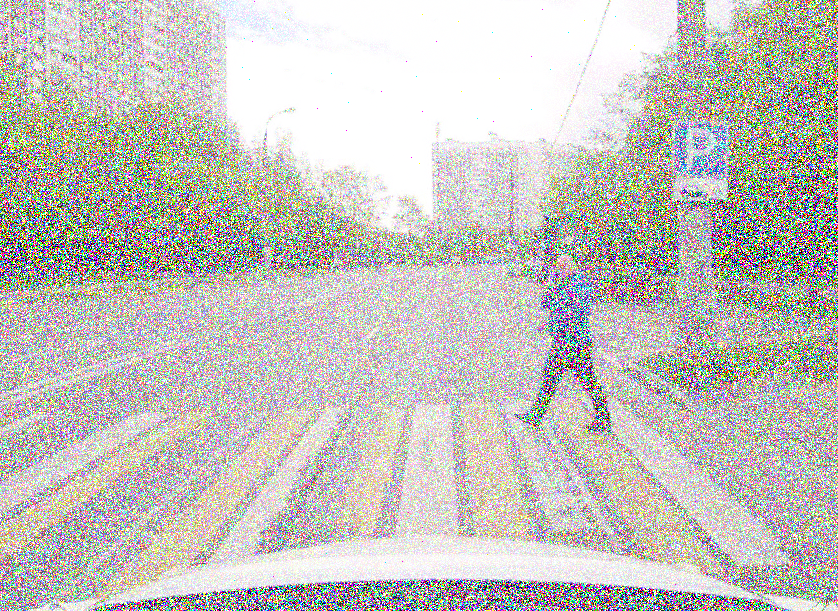
\includegraphics[width=\textwidth]{../outputs/image_impulse_noise.png}
    \caption{Изображение с импульсным шумом}
    \label{fig:impulse_image}
\end{figure}

\pagebreak

\subsection{Мультипликативный шум}

Мультипликативный шум описывается следующим выражени-
ем:
\begin{equation}
    I_{new} = I(x, y) * \eta(x, y), 
\label{eq:complex_func}
\end{equation}
где $I_{new}$ — зашумленное изображение, $I$ — исходное изображение,
$\eta$ — не зависящий от сигнала мультипликативный шум, умножающий зарегистрированный сигнал. 
В качестве примера можно привести зернистость фотопленки, ультразвуковые изображения и т.д.
Частным случаем мультипликативного шума является спекл-шум,
который появляется на изображениях, полученных устройствами
с когерентным формированием изображений, например, медицинскими сканерами или радарами.
На таких изображениях можно отчетливо наблюдать светлые пятна, крапинки (спеклы), которые
разделены темными участками изображения.
  
\pagebreak

\begin{lstlisting}[style=cpp_white, caption={Исходный код для применения мультипликативного шума к изображению}]
double var = 0.05;
std::vector<cv::Mat> image_out_BGR;

cv::split(image, image_out_BGR);

for(int i = 0; i < image_out_BGR.size(); ++i){

    cv::Mat gauss(image_out_BGR[i].size(), CV_32F);
    cv::randn(gauss, cv::Scalar(0), cv::Scalar(cv::sqrt(var)));

    if( image_out_BGR[i].depth() == CV_8U){
        cv::Mat image_out_BGR_f;

        image_out_BGR[i].convertTo(image_out_BGR_f, CV_32F);

        image_out_BGR_f += image_out_BGR_f.mul(gauss);
        image_out_BGR_f.convertTo(image_out_BGR[i], image_out_BGR[i].type());
    } else
        image_out_BGR[i] += image_out_BGR[i].mul(gauss);
}

cv::merge(image_out_BGR, image_out);
\end{lstlisting}

\begin{figure}[ht]
    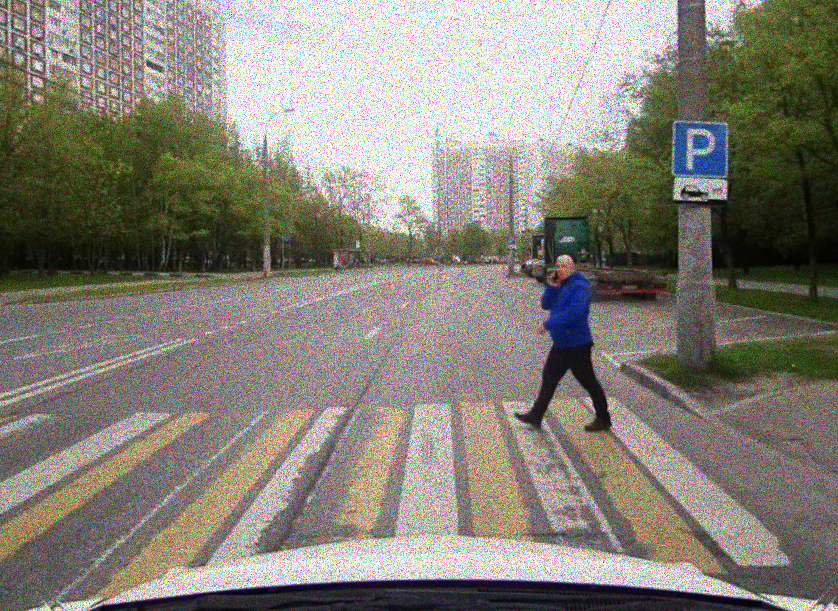
\includegraphics[width=\textwidth]{../outputs/image_mltp_noise.png}
    \caption{Изображение с мультипликативным шумом}
    \label{fig:impulse_image}
\end{figure}

\pagebreak

\subsection{Гауссов (нормальный) шум}

Гауссов шум на изображении может возникать в следствие недостатка освещенности сцены, 
высокой температуры и т.д. Модельшума широко распространена в задачах низкочастотной 
фильтрации изображений. Функция распределения плотности вероятности
$p(z)$ случайной величины $z$ описывается следующим выражением:

\begin{equation}
    p(z) = \frac{1}{\sigma \sqrt(2\pi)} e ^{\frac{(-x-\mu)^2}{2\sigma^2}}
\label{eq:complex_func}
\end{equation}

где $z$ — интенсивность изображения (например, для полутоново-
го изображения $z \in [0,255]$), $\mu$ — среднее (математическое ожи-
дание) случайной величины $z$, $\sigma$ — среднеквадратичное отклоне-
ние, дисперсия $\sigma ^ 2$ определяет мощность вносимого шума.
  
\pagebreak

\begin{lstlisting}[style=cpp_white, caption={Исходный код для применения Гауссовского (нормального) шума к изображению}]
double mean = 0;
double var = 0.05;
std::vector<cv::Mat> image_out_BGR;

cv::split(image, image_out_BGR);

for(int i = 0; i < image_out_BGR.size(); ++i){

    cv::Mat gauss(image_out_BGR[i].size(), CV_32F);
    cv::randn(gauss, cv::Scalar(mean), cv::Scalar(cv::sqrt(var)));

    if( image_out_BGR[i].depth() == CV_8U){
        cv::Mat image_out_BGR_f;

        image_out_BGR[i].convertTo(image_out_BGR_f, CV_32F);

        image_out_BGR_f += gauss * 255;
        image_out_BGR_f.convertTo(image_out_BGR[i], image_out_BGR[i].type());
    } else
        image_out_BGR[i] += gauss;
}

cv::merge(image_out_BGR, image_out);
\end{lstlisting}

\begin{figure}[ht]
    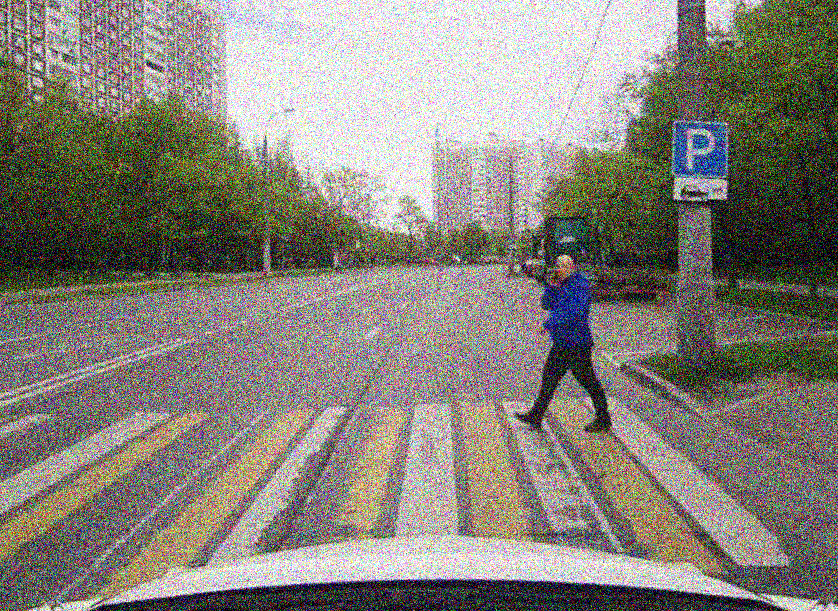
\includegraphics[width=\textwidth]{../outputs/image_gauss_noise.png}
    \caption{Изображение с Гауссовским (нормальным) шумом}
    \label{fig:impulse_image}
\end{figure}

\pagebreak

\subsection{Шум квантования}

Зависит от выбранного шага квантования и самого сигнала.
Шум квантования может приводить, например, к появлению ложных контуров 
вокруг объектов или убирать слабо контрастные детали на изображении. Такой шум не устраняется.


\begin{lstlisting}[style=cpp_white, caption={Исходный код для применения шума квантования к изображению}]
if(image.depth() == CV_8U)
    image.convertTo(image_out, CV_32F, 1.0 / 255);
else
    image_out = image.clone();

size_t vals = unique(image_out).size();
vals = static_cast<size_t>(cv::pow(2, ceil(log2(vals))));

int rows = image_out.rows;
int cols = image_out.cols * image_out.channels();

if(image_out.isContinuous()){
    cols *= rows;
    rows = 1;
}

using param_t = std::poisson_distribution<int>::param_type;
std::default_random_engine engine;
std::poisson_distribution<> poisson;

for(int i = 0; i < rows; ++i){
    float* ptr = image_out.ptr<float>(i);
    for(int j = 0; j < cols; ++j)
        ptr[j] = float(poisson(engine, param_t({ptr[j] * vals}))) / vals;
}

if(image.depth() == CV_8U)
    image_out.convertTo(image_out, CV_8U, 255);
\end{lstlisting}

\begin{figure}[ht]
    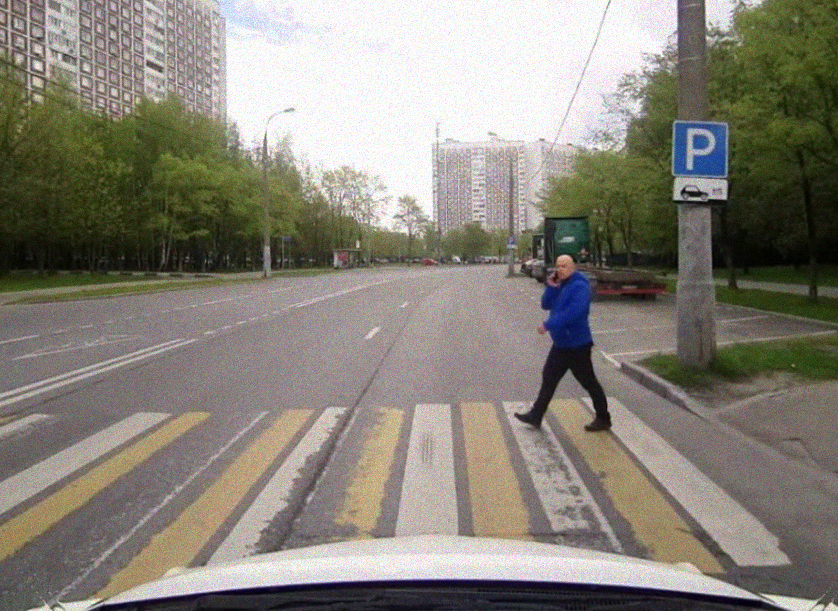
\includegraphics[width=\textwidth]{../outputs/image_quant_noise.png}
    \caption{Изображение с шумом квантования}
    \label{fig:impulse_image}
\end{figure}

\pagebreak

\section{Низкочастотная фильтрация}

\subsection{Контргармонический усредняющий фильтр}

Фильтр базируется на выражении:

\begin{equation}
    I_{new}(x, y) = \frac{\sum_{i=0}^{m}\sum_{j=0}^{n} I(i, j) ^ {Q+1}}{\sum_{i=0}^{m}\sum_{j=0}^{n} I(i, j) ^ Q}
\label{eq:complex_func}
\end{equation}

где $Q$ — порядок фильтра. Контргармонический фильтр является
обобщением усредняющих фильтров и при $Q$ > 0 подавляет шумы
типа «перец», а при $Q$ < 0 — шумы типа «соль», однако одновременное удаление 
белых и черных точек невозможно. При $Q$ = 0 фильтр превращается в арифметический, 
а при $Q$ = -1 — в гармонический.

Какой-то brutforce получился... Можно оптимизровать с помощью интегральных \href{https://en.wikipedia.org/wiki/Summed-area_table}{выражений} или же посмотреть более простые \href{https://github.com/BBuf/Image-processing-algorithm}{оптимизации}

\begin{lstlisting}[style=cpp_white, caption={Исходный код для контргармонического усредняющего фильтра}]
image = cv::imread(path + "/lab3/outputs/image_quant_noise.png", 1);

std::pair<int, int> kernel = std::make_pair(2, 2);
const int Q = -1;

image_out = image;
std::cout << image.channels();

int radius_c = (kernel.first - 1) / 2;  // columns offset
int radius_r = (kernel.second - 1) / 2; // rows offset
float res1 = 0, res2 = 0;


for(int c = 0; c < image.channels(); ++c){
    for (int i = radius_r; i < image.rows - kernel.second - 1; i++){
        for (int j = radius_c; j < image.cols - kernel.first - 1; j++)
        {
            res1 = 0; res2 = 0;

            for (int m = 0; m < kernel.first; ++m)
            {
                for (int n = 0; n < kernel.second; ++n)
                {
                    res1 += pow(image.at<cv::Vec3b>(i + m, j + n)[c], Q + 1);
                    res2 += pow(image.at<cv::Vec3b>(i + m, j + n)[c], Q);
                }
            }

            image_out.at<cv::Vec3b>(i, j)[c] = res1 / res2;                                                            
        }
    }
}

cv::imwrite(path + "/lab3/addition/image_quant_countergarmonic_filter_Q1.png", image_out);
cv::imshow("Image", image_out);
cv::waitKey(0);
\end{lstlisting}

Применим к изображению с импульссивным шумом контргармонический усредняющий фильтр с ядром 2*2:

\begin{figure}[hbt!]
    \centering
    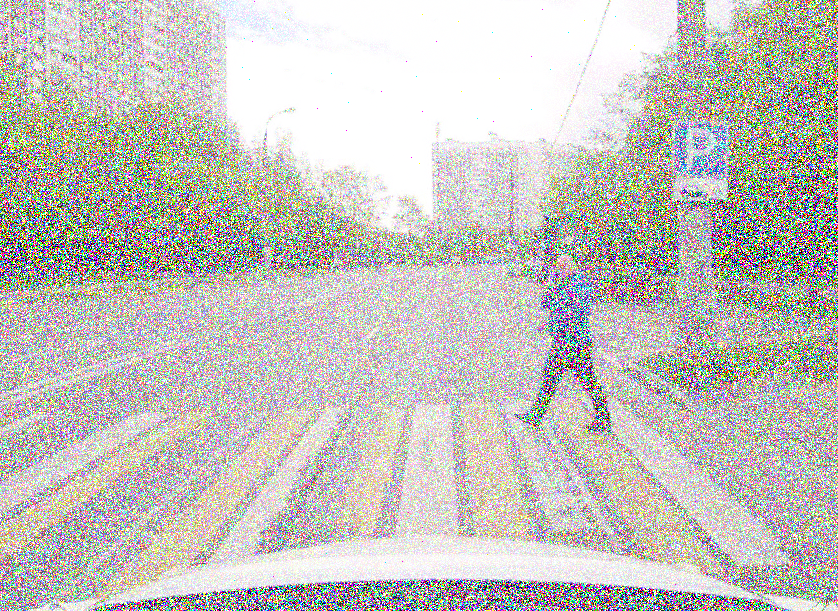
\includegraphics[width=0.6\textwidth]{../outputs/image_impulse_noise.png}
    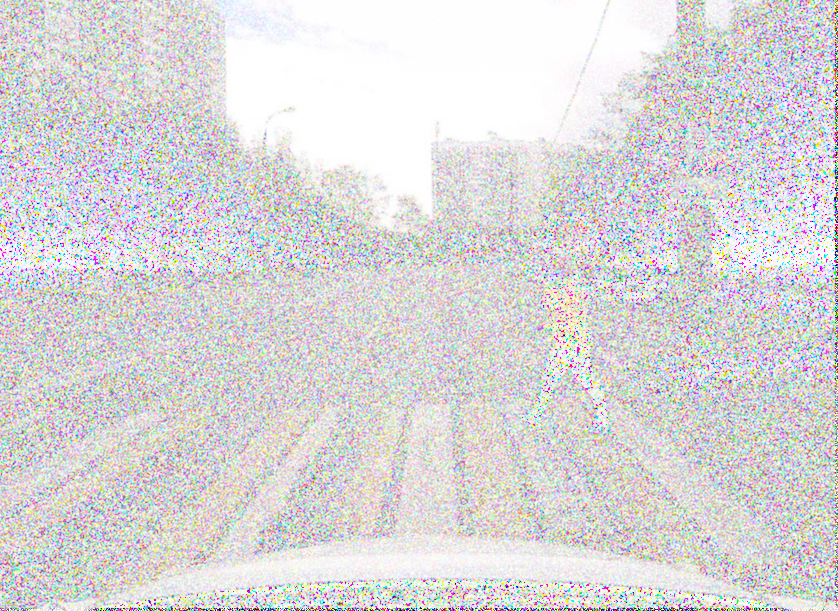
\includegraphics[width=0.6\textwidth]{../addition/image_impulse_countergarmonic_filter_Q1.png}
    \caption{Изображение с импульсивным шумом до и после применения контргармонического усредняющего фильтра с Q = 1}
    \label{fig:stich_images}
\end{figure}

Применим к изображению с мультипликативным шумом контргармонический усредняющий фильтр с ядром 2*2:

\begin{figure}[hbt!]
    \centering
    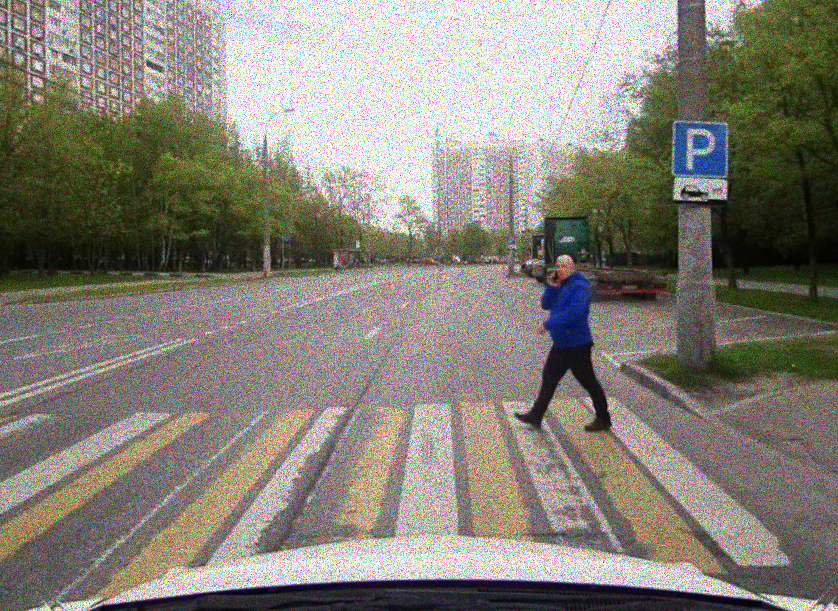
\includegraphics[width=0.6\textwidth]{../outputs/image_mltp_noise.png}
    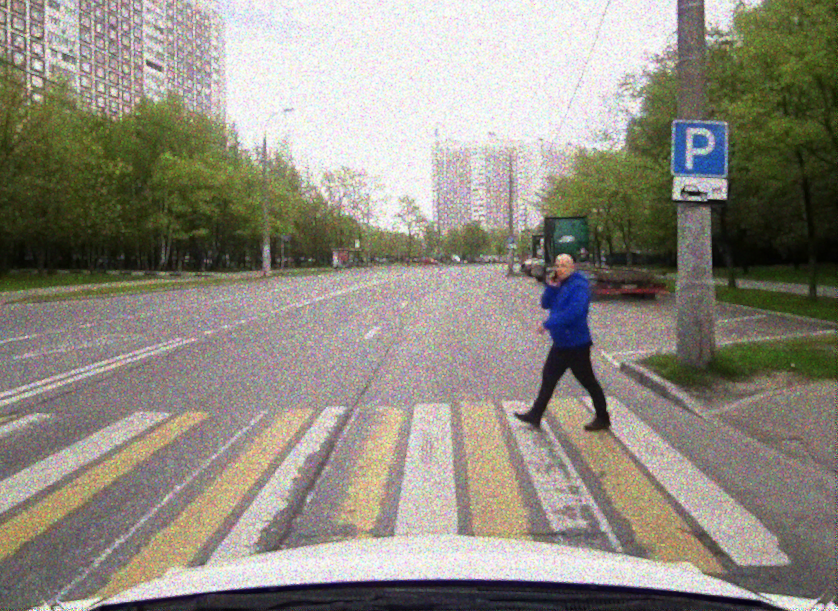
\includegraphics[width=0.6\textwidth]{../addition/image_mltp_countergarmonic_filter_Q3.png}
    \caption{Изображение с мультипликативным шумом до и после применения контргармонического усредняющего фильтра с Q = 3}
    \label{fig:stich_images}
\end{figure}

Применим к изображениям с гауссовским шумом контргармонический усредняющий фильтр с ядром 2*2:

\begin{figure}[hbt!]
    \centering
    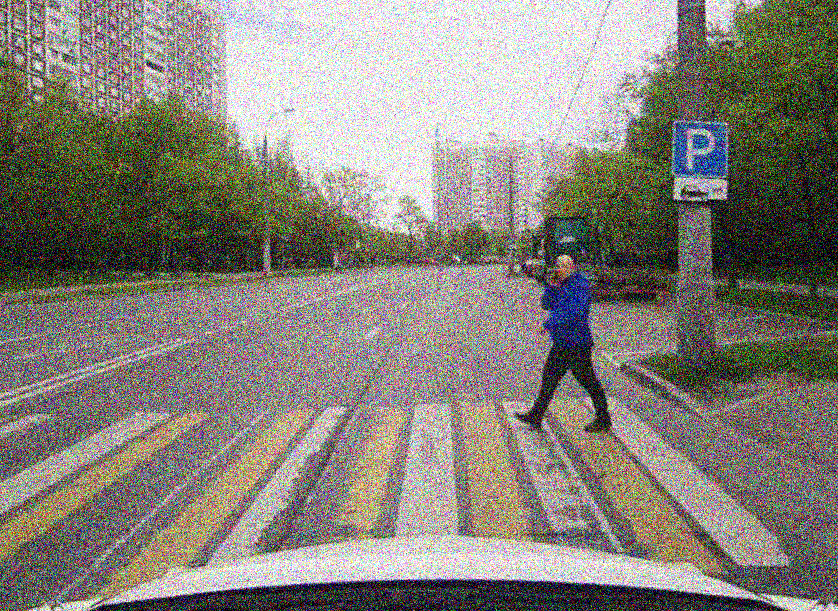
\includegraphics[width=0.6\textwidth]{../outputs/image_gauss_noise.png}
    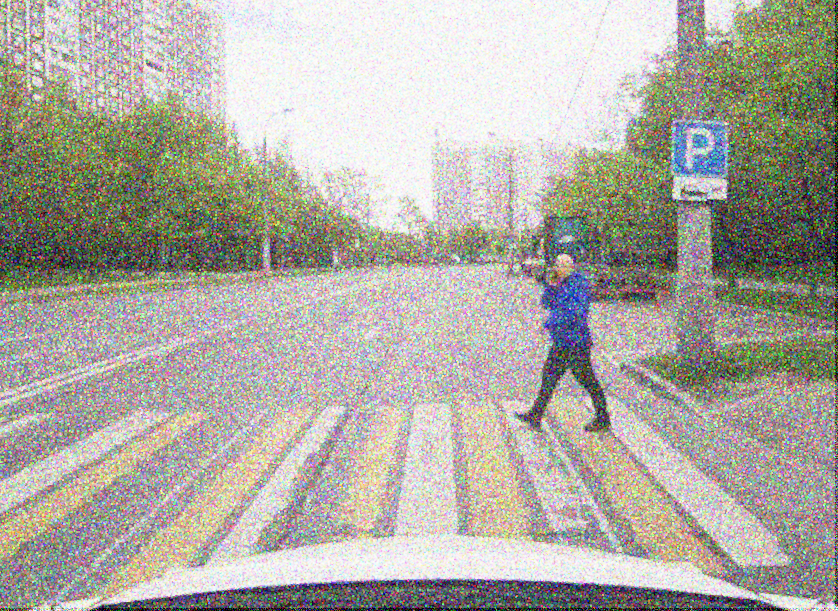
\includegraphics[width=0.6\textwidth]{../addition/image_gauss_countergarmonic_filter_Q5.png}
    \caption{Изображение с гауссовским шумом до и после применения контргармонического усредняющего фильтра с Q = 5}
    \label{fig:stich_images}
\end{figure}

\pagebreak
Применим к изображениям с шумом квантизации контргармонический усредняющий фильтр с ядром 2*2:

\begin{figure}[ht]
    \centering
    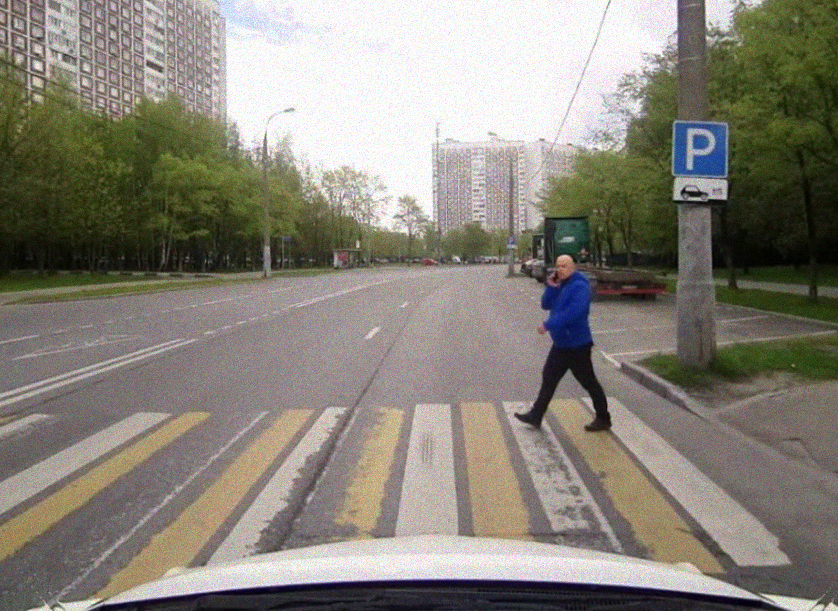
\includegraphics[width=0.6\textwidth]{../outputs/image_quant_noise.png}
    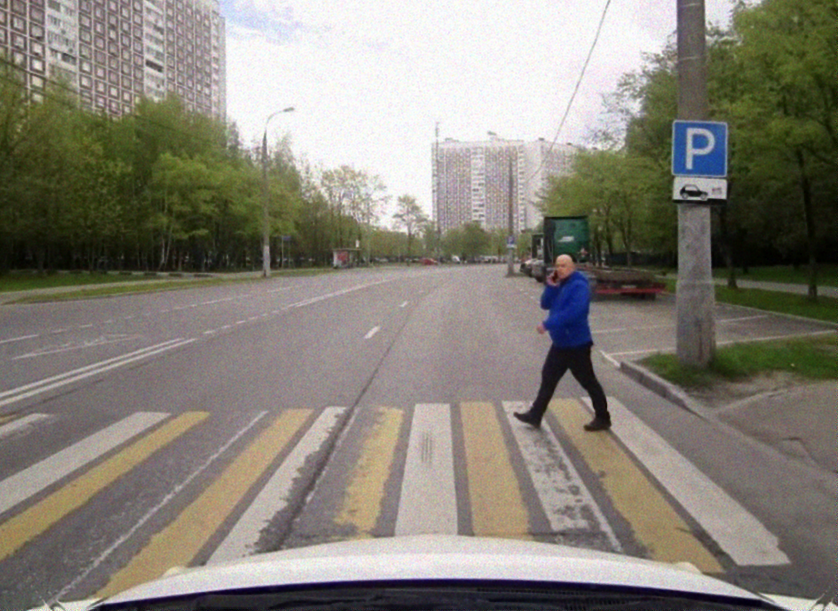
\includegraphics[width=0.6\textwidth]{../addition/image_quant_countergarmonic_filter_Q1.png}
    \caption{Изображение с шумом квантизации до и после применения контргармонического усредняющего фильтра с Q = 1}
    \label{fig:stich_images}
\end{figure}


\pagebreak



\subsection{Фильтр Гаусса}

Пиксели в скользящем окне, расположенные ближе к анализируемому пикселю, должны оказывать большее влияние на результат 
фильтрации, чем крайние. Поэтому коэффициенты весов маски можно описать колоколообразной функцией Гаусса (3). При
фильтрации изображений используется двумерный фильтр Гаусса:



\begin{equation}
    G_\sigma = \frac{1}{2\pi\sigma^2} e ^{\frac{-x^2-y^2}{2\sigma^2}}
\label{eq:complex_func}
\end{equation}

где $Q$ — порядок фильтра. Контргармонический фильтр является
обобщением усредняющих фильтров и при $Q$ > 0 подавляет шумы
типа «перец», а при $Q$ < 0 — шумы типа «соль», однако одновременное удаление 
белых и черных точек невозможно. При $Q$ = 0 фильтр превращается в арифметический, 
а при $Q$ = -1 — в гармонический.

\begin{lstlisting}[style=cpp_white, caption={Исходный код фильра Гаусса}]
image = cv::imread(path + "/lab3/outputs/image_quant_noise.png", 1);
cv::GaussianBlur(image, image_out, cv::Size(5, 5), 0);
\end{lstlisting}

Применим к изображению с импульссивным шумом фильтр Гаусса с ядром 3*3:

\begin{figure}[hbt!]
    \centering
    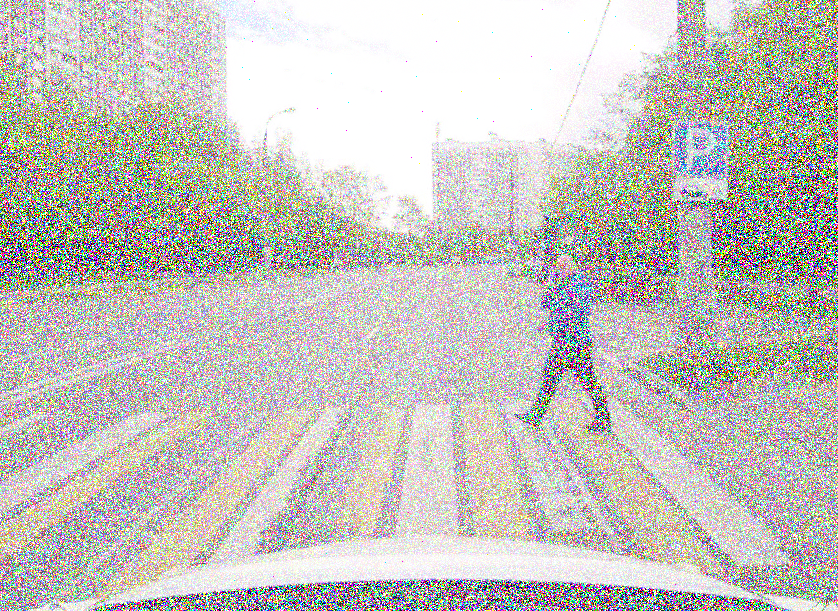
\includegraphics[width=0.6\textwidth]{../outputs/image_impulse_noise.png}
    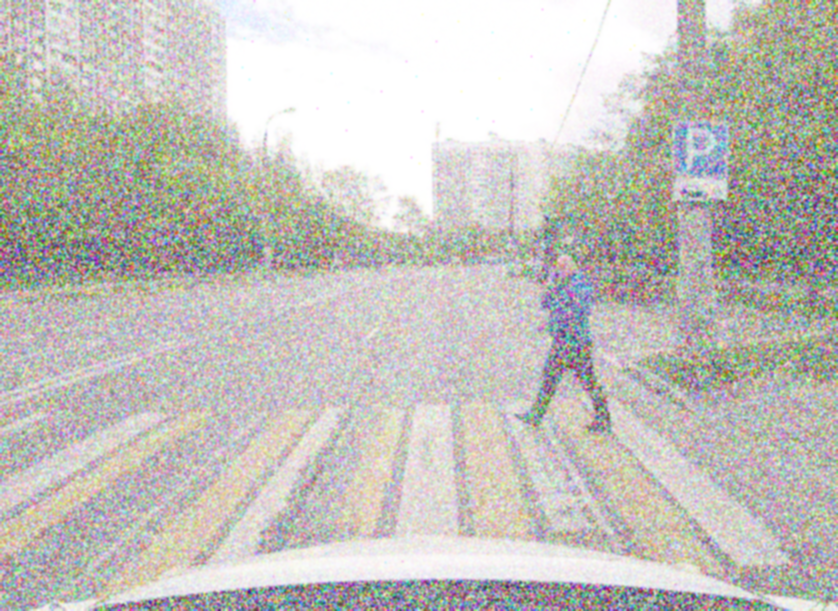
\includegraphics[width=0.6\textwidth]{../outputs/image_impulse_filter.png}
    \caption{Изображение с импульсивным шумом до и после применения фильтра Гаусса}
    \label{fig:stich_images}
\end{figure}

Применим к изображению с мультипликативным шумом фильтр Гаусса с ядром 3*3:

\begin{figure}[hbt!]
    \centering
    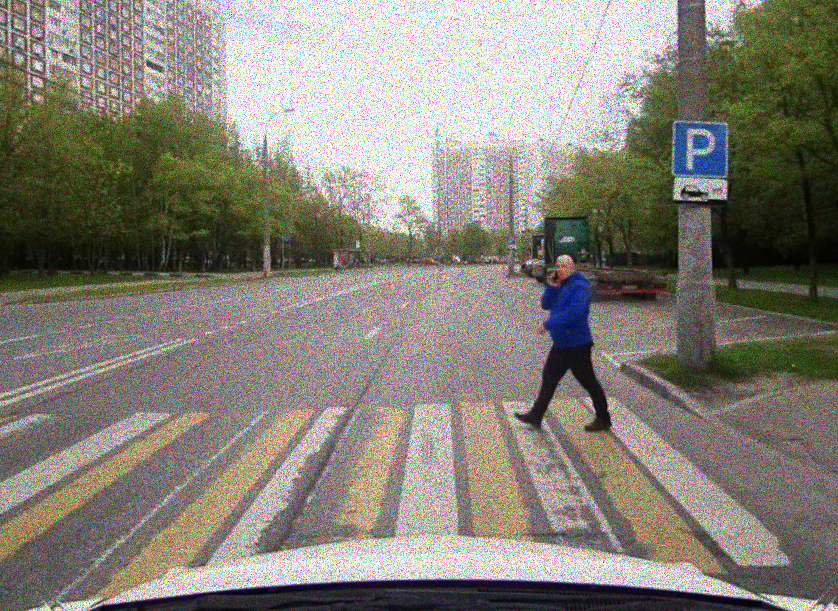
\includegraphics[width=0.6\textwidth]{../outputs/image_mltp_noise.png}
    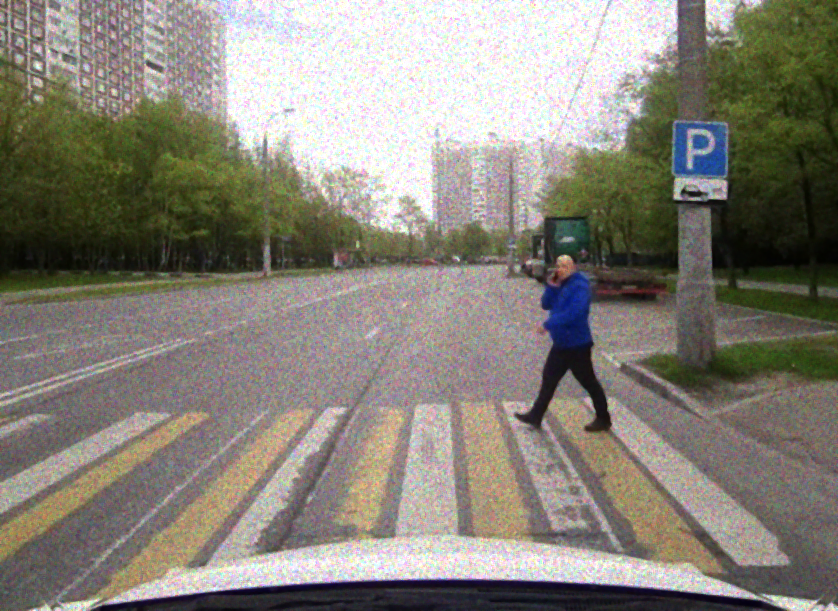
\includegraphics[width=0.6\textwidth]{../addition/image_mltp_median_filter_k3.png}
    \caption{Изображение с мультипликативным шумом до и после применения фильтра Гаусса}
    \label{fig:stich_images}
\end{figure}

\pagebreak
Применим к изображениям с гауссовским шумом фильтр Гаусса с ядром 3*3:

\begin{figure}[hbt!]
    \centering
    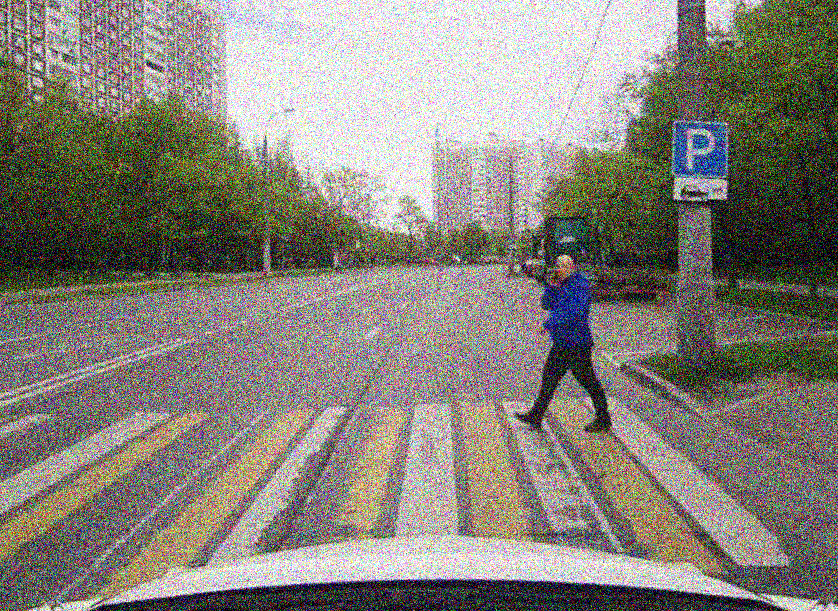
\includegraphics[width=0.6\textwidth]{../outputs/image_gauss_noise.png}
    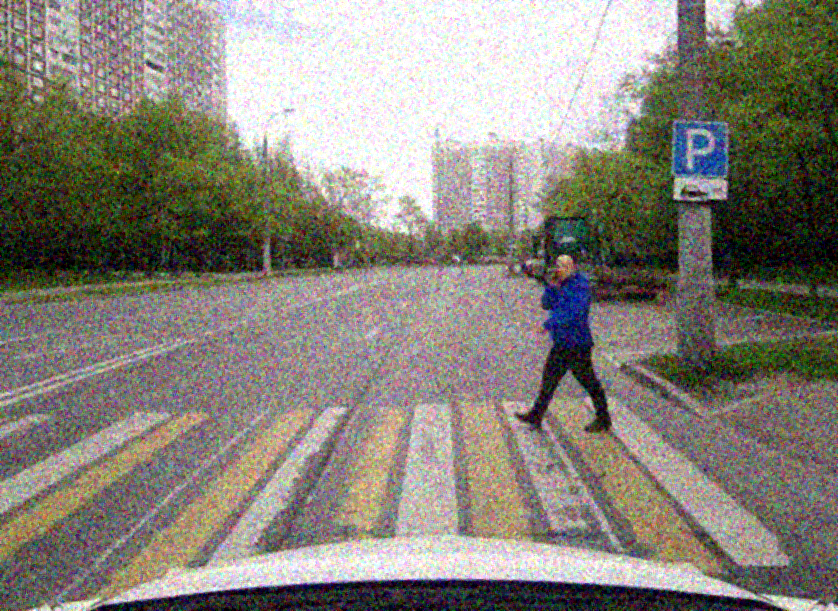
\includegraphics[width=0.6\textwidth]{../addition/image_gauss_median_filter_k3.png}
    \caption{Изображение с гауссовским шумом до и после применения фильтра Гаусса}
    \label{fig:stich_images}
\end{figure}

\pagebreak
Применим к изображениям с шумом квантизации фильтр Гаусса с ядром 3*3:

\begin{figure}[ht]
    \centering
    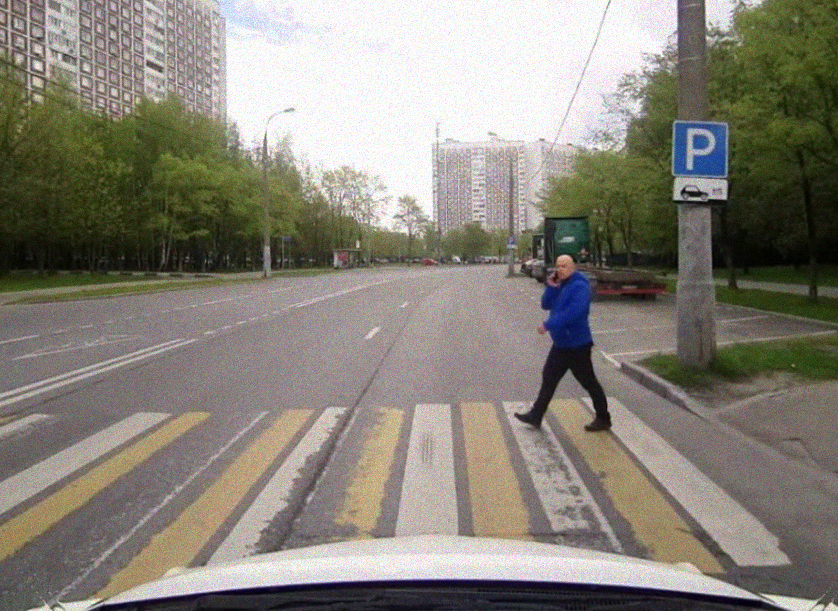
\includegraphics[width=0.6\textwidth]{../outputs/image_quant_noise.png}
    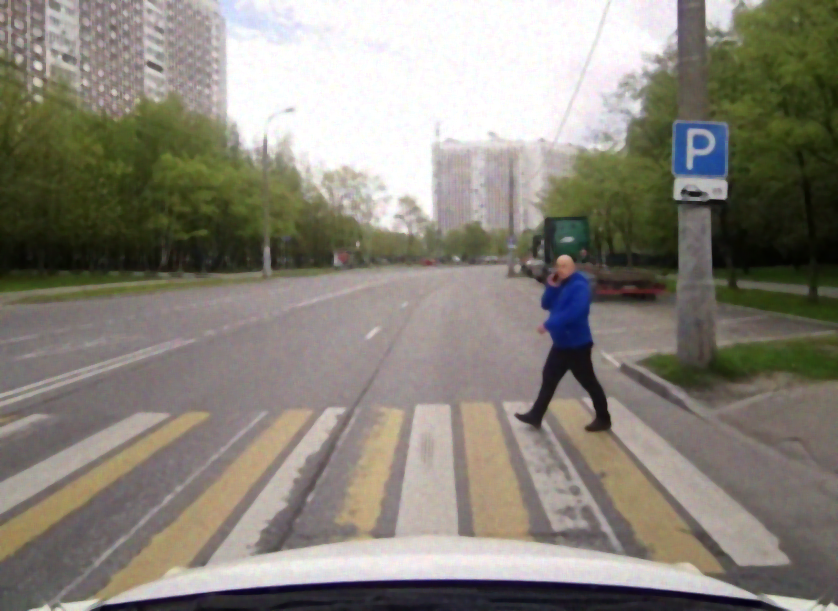
\includegraphics[width=0.6\textwidth]{../addition/image_quant_median_filter_k5.png}
    \caption{Изображение с шумом квантизации до и после применения фильтра Гаусса}
    \label{fig:stich_images}
\end{figure}



\pagebreak

\section{Нелинейная фильтрация}

\subsection{Медианная фильтрация}

В классическом медианном фильтре используется маска с единичными коэффициентами. Произвольная форма окна 
может задаваться при помощи нулевых коэффициентов. Значения интенсивностей пикселей в окне представляются 
в виде вектора-столбца и сортируются по возрастанию. Отфильтрованному пикселю при-
свается медианное (среднее) в ряду значение интенсивности. Номер медианного элемента после сортировки может быть вычислен
по формуле 

\begin{equation}
    n = \frac{N + 1}{2},
\label{eq:complex_func}
\end{equation}

где $N$ — число пикселей, участвующих в сортировке.

\begin{lstlisting}[style=cpp_white, caption={Исходный код медианного фильтра}]
image = cv::imread(path + "/lab3/outputs/image_gauss_noise.png", 1);

cv::medianBlur(image, image_out, 3);
\end{lstlisting}
\pagebreak

Применим к изображению с импульссивным шумом медианный фильтр с ядром 3*3:

\begin{figure}[hbt!]
    \centering
    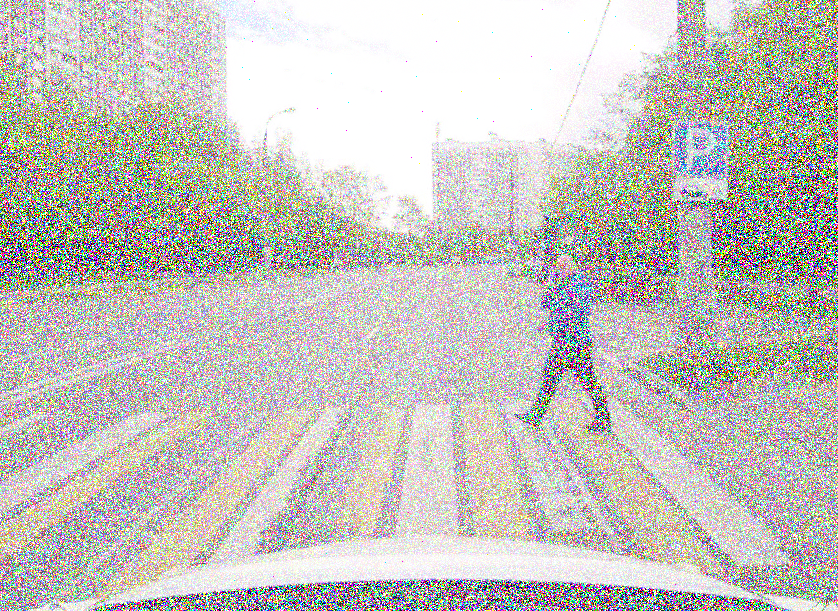
\includegraphics[width=0.6\textwidth]{../outputs/image_impulse_noise.png}
    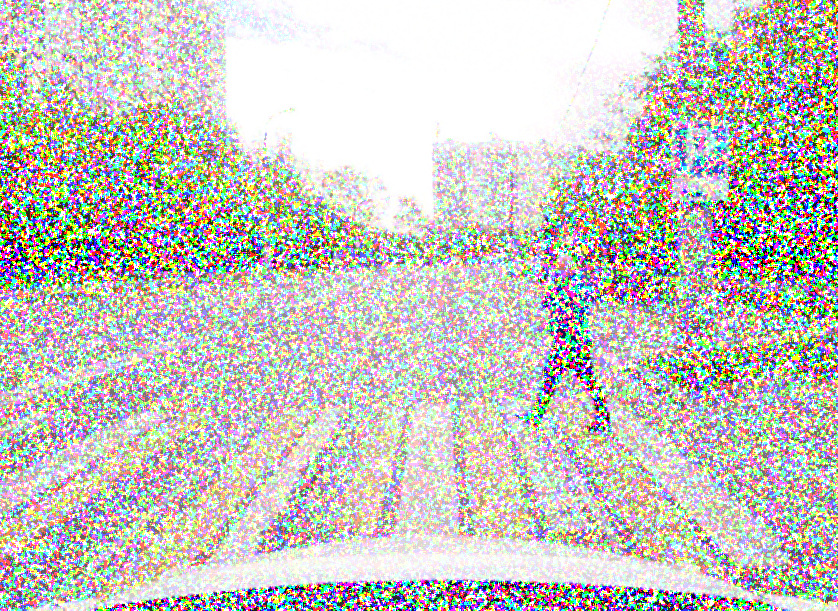
\includegraphics[width=0.6\textwidth]{../addition/image_impulse_median_filter_k3.png}
    \caption{Изображение с импульсивным шумом до и после применения медианного фильтра}
    \label{fig:stich_images}
\end{figure}

Применим к изображению с мультипликативным шумом медианный фильтр с ядром 3*3:

\begin{figure}[hbt!]
    \centering
    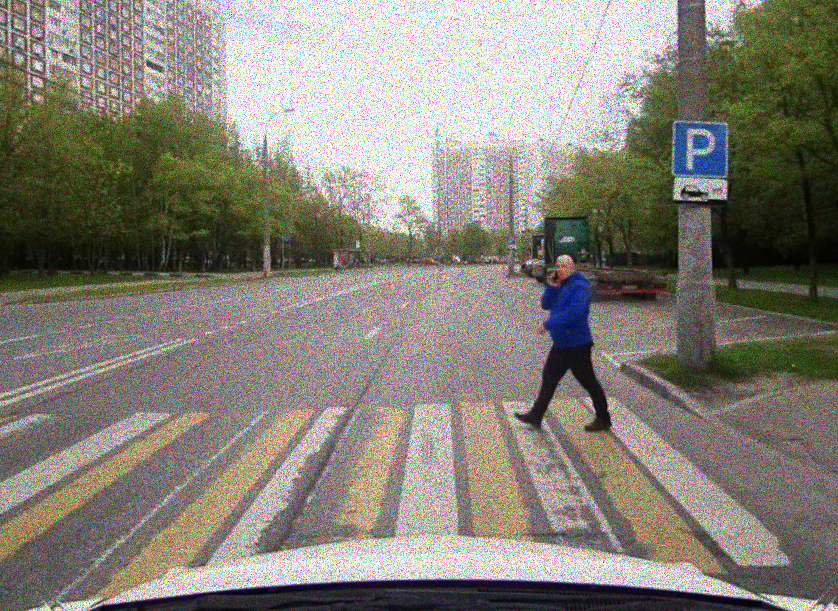
\includegraphics[width=0.6\textwidth]{../outputs/image_mltp_noise.png}
    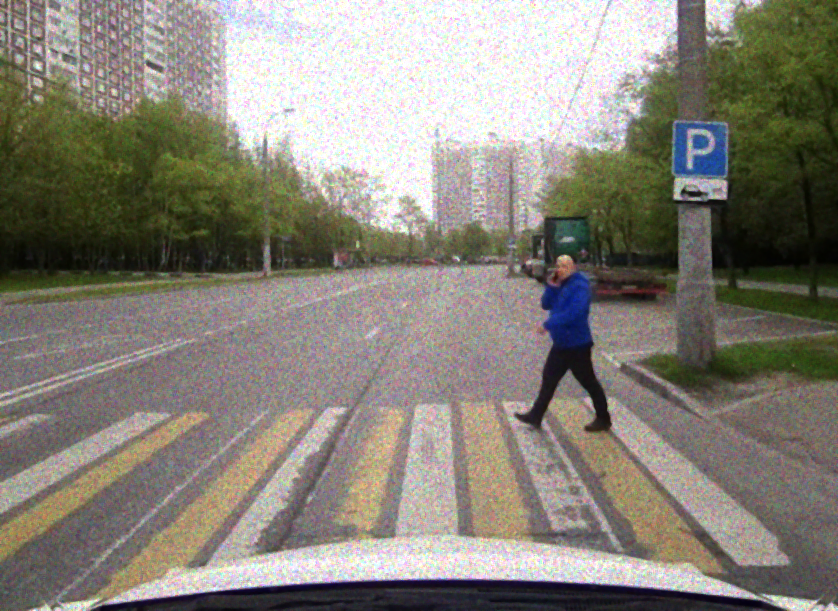
\includegraphics[width=0.6\textwidth]{../addition/image_mltp_median_filter_k3.png}
    \caption{Изображение с мультипликативным шумом до и после применения медианного фильтра}
    \label{fig:stich_images}
\end{figure}

\pagebreak
Применим к изображениям с гауссовским шумом медианный фильтр с ядром 3*3:

\begin{figure}[hbt!]
    \centering
    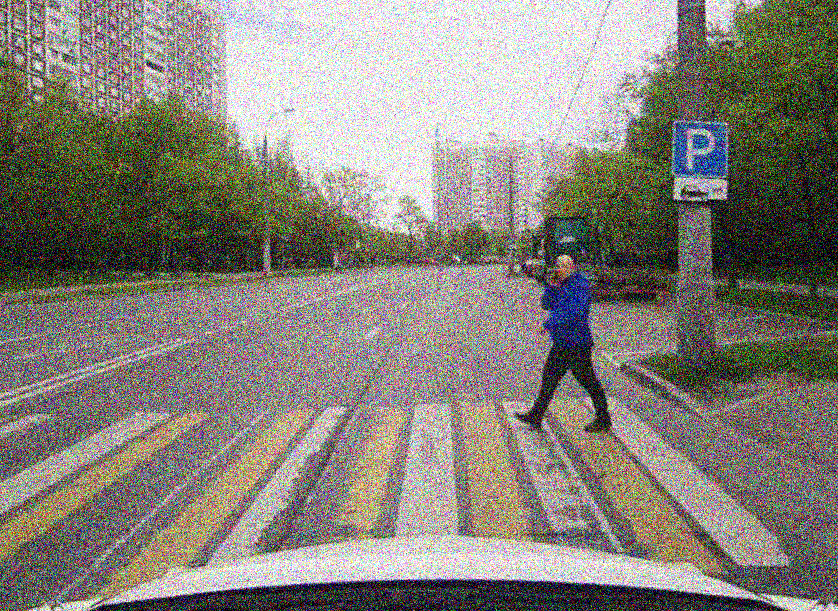
\includegraphics[width=0.6\textwidth]{../outputs/image_gauss_noise.png}
    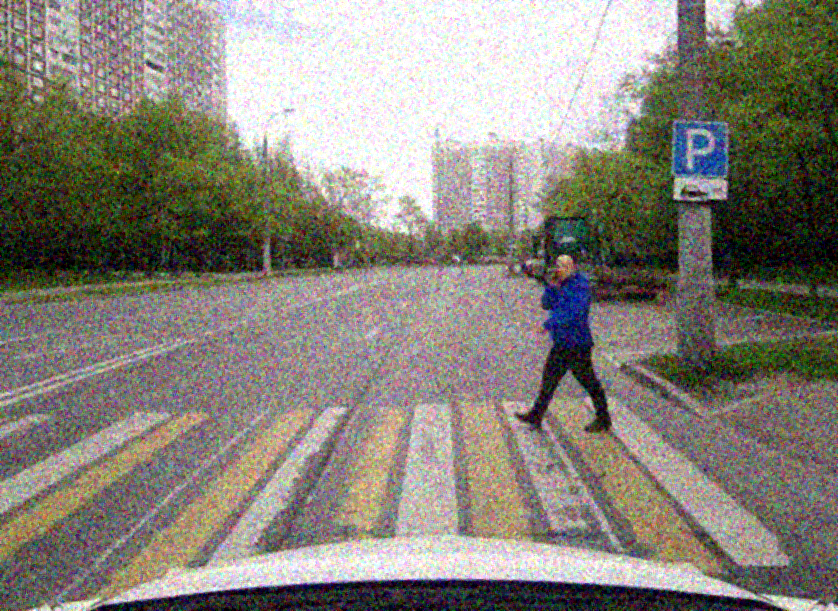
\includegraphics[width=0.6\textwidth]{../addition/image_gauss_median_filter_k3.png}
    \caption{Изображение с гауссовским шумом до и после применения медианного фильтра}
    \label{fig:stich_images}
\end{figure}

\pagebreak
Применим к изображениям с шумом квантизации медианный фильтр с ядром 3*3:

\begin{figure}[ht]
    \centering
    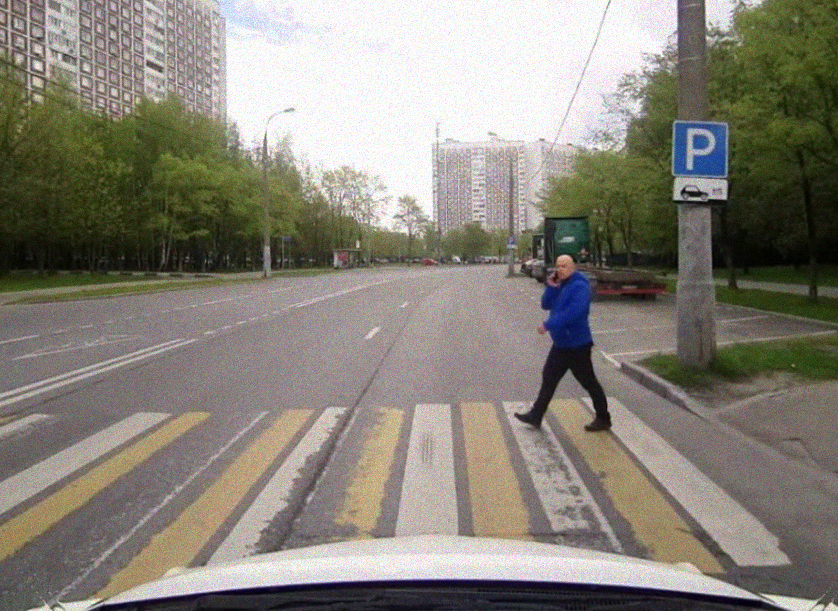
\includegraphics[width=0.6\textwidth]{../outputs/image_quant_noise.png}
    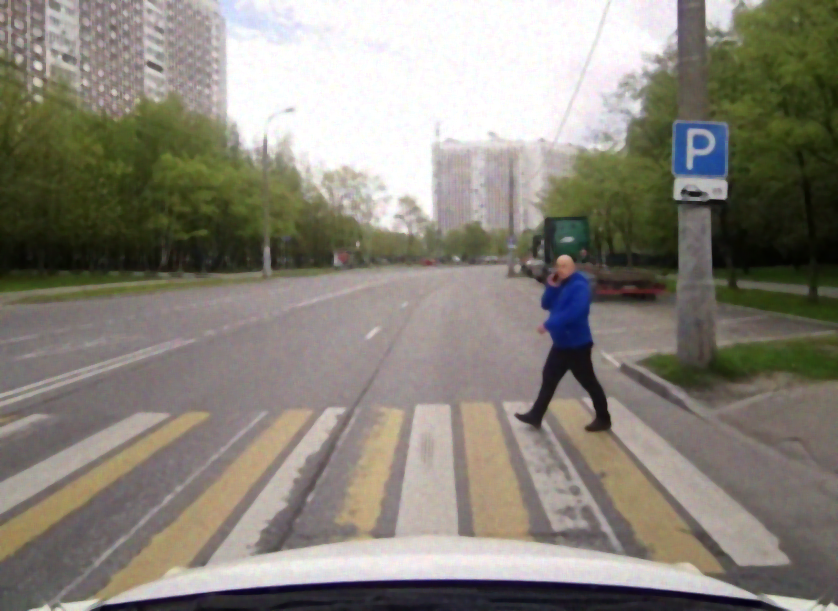
\includegraphics[width=0.6\textwidth]{../addition/image_quant_median_filter_k5.png}
    \caption{Изображение с шумом квантизации до и после применения медианного фильтра}
    \label{fig:stich_images}
\end{figure}

\pagebreak

Применим к изображению с импульссивным шумом медианный фильтр с ядром 5*5:

\begin{figure}[hbt!]
    \centering
    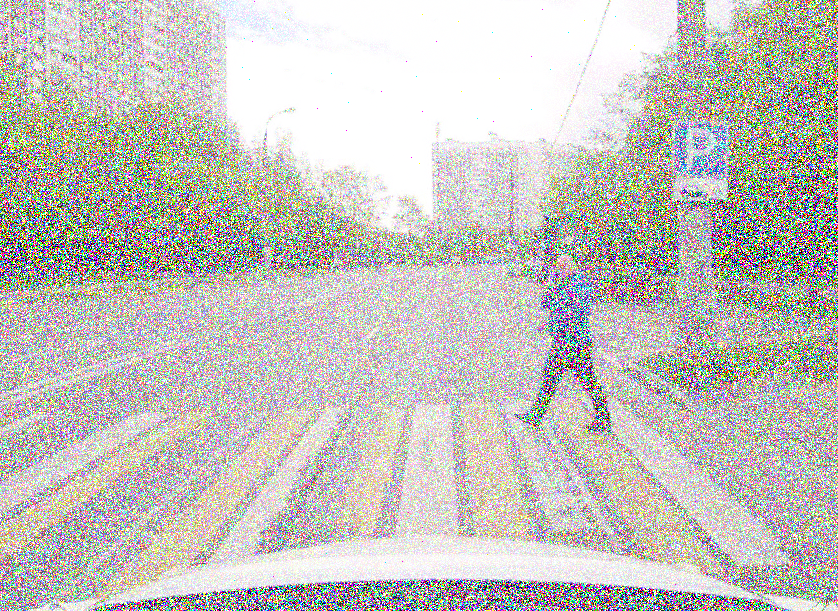
\includegraphics[width=0.6\textwidth]{../outputs/image_impulse_noise.png}
    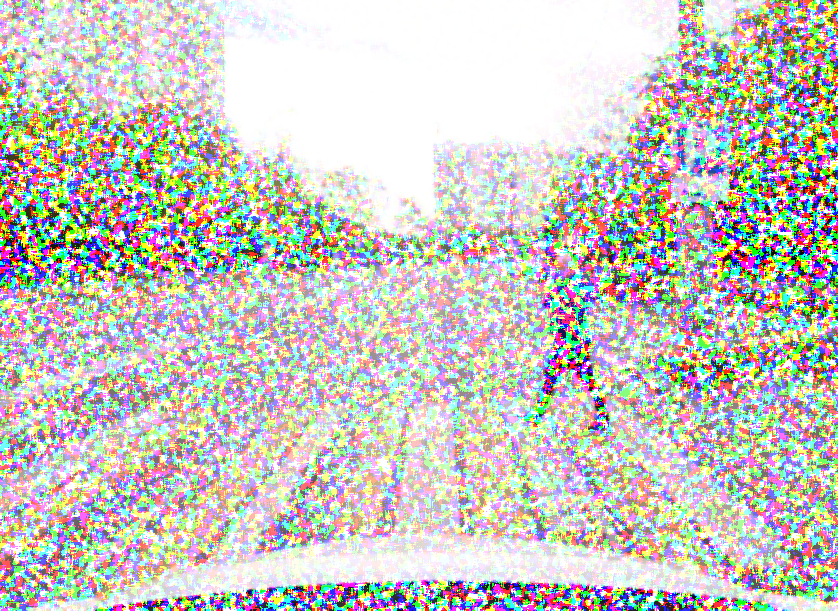
\includegraphics[width=0.6\textwidth]{../addition/image_impulse_median_filter_k5.png}
    \caption{Изображение с импульсивным шумом до и после применения медианного фильтра}
    \label{fig:stich_images}
\end{figure}

\pagebreak
Применим к изображению с мультипликативным шумом медианный фильтр с ядром 5*5:

\begin{figure}[hbt!]
    \centering
    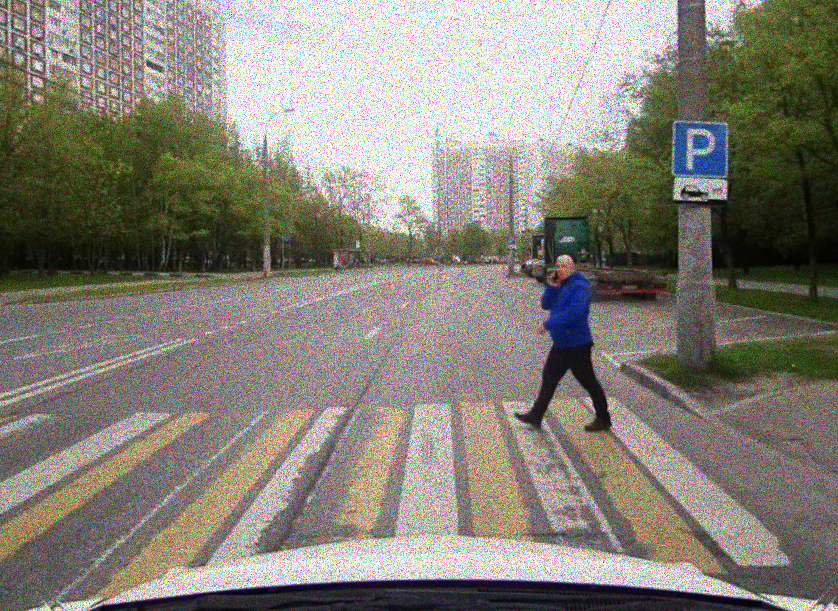
\includegraphics[width=0.6\textwidth]{../outputs/image_mltp_noise.png}
    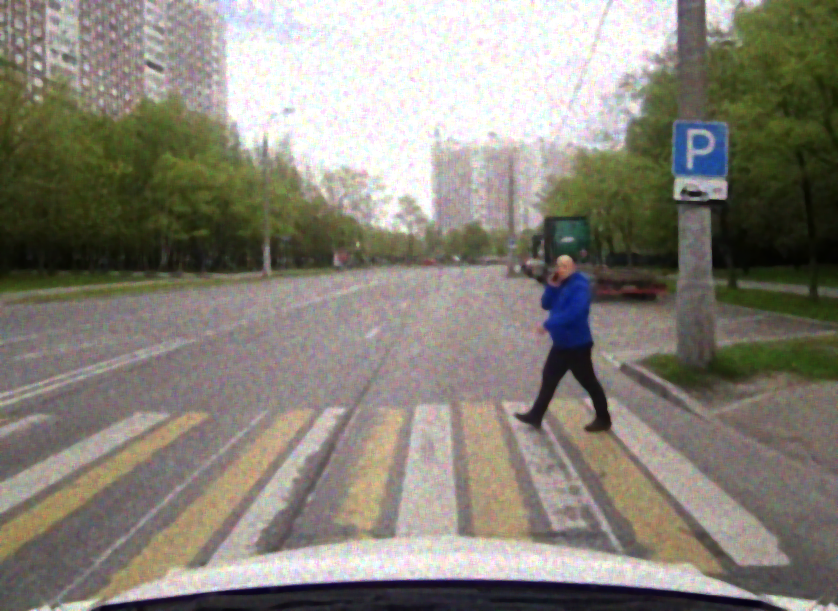
\includegraphics[width=0.6\textwidth]{../addition/image_mltp_median_filter_k5.png}
    \caption{Изображение с мультипликативным шумом до и после применения медианного фильтра}
    \label{fig:stich_images}
\end{figure}

\pagebreak
Применим к изображениям с гауссовским шумом медианный фильтр с ядром 5*5:

\begin{figure}[hbt!]
    \centering
    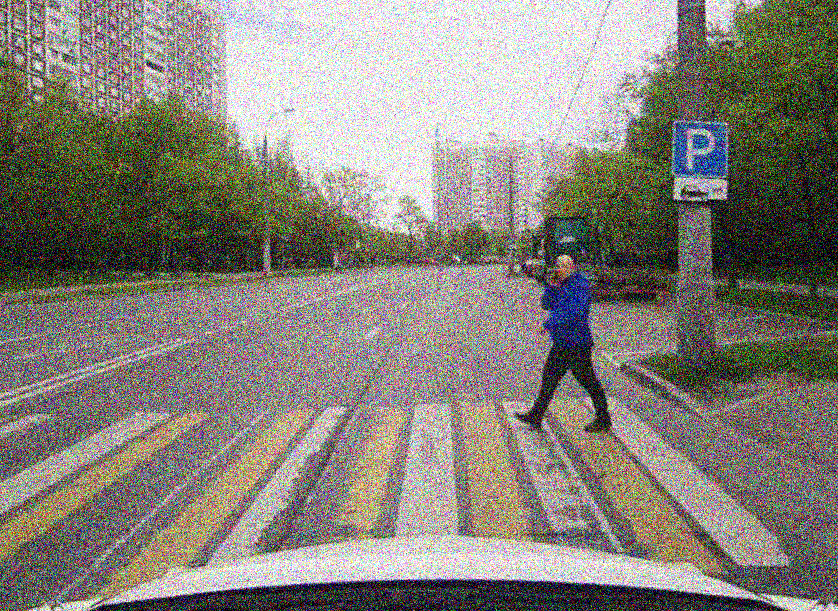
\includegraphics[width=0.6\textwidth]{../outputs/image_gauss_noise.png}
    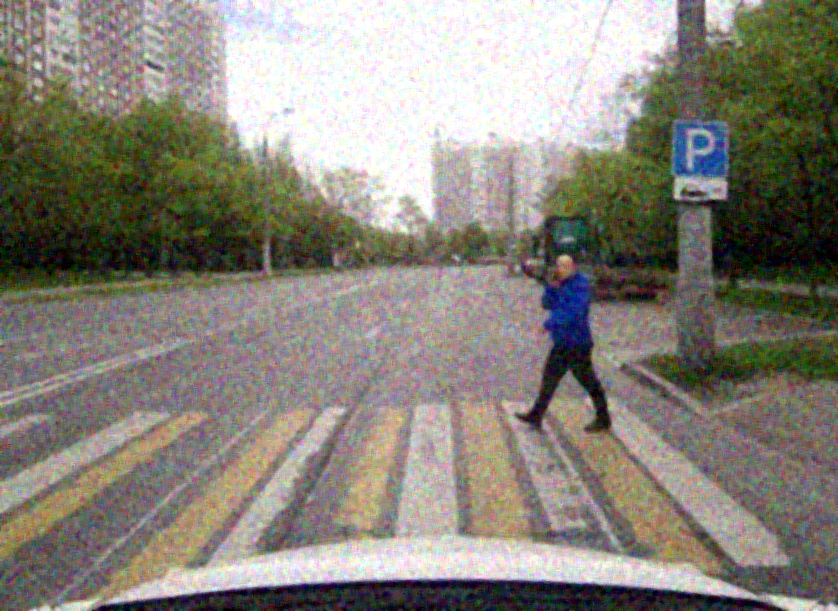
\includegraphics[width=0.6\textwidth]{../addition/image_gauss_median_filter_k5.png}
    \caption{Изображение с гауссовским шумом до и после применения медианного фильтра}
    \label{fig:stich_images}
\end{figure}

\pagebreak
Применим к изображениям с шумом квантизации медианный фильтр с ядром 5*5:

\begin{figure}[ht]
    \centering
    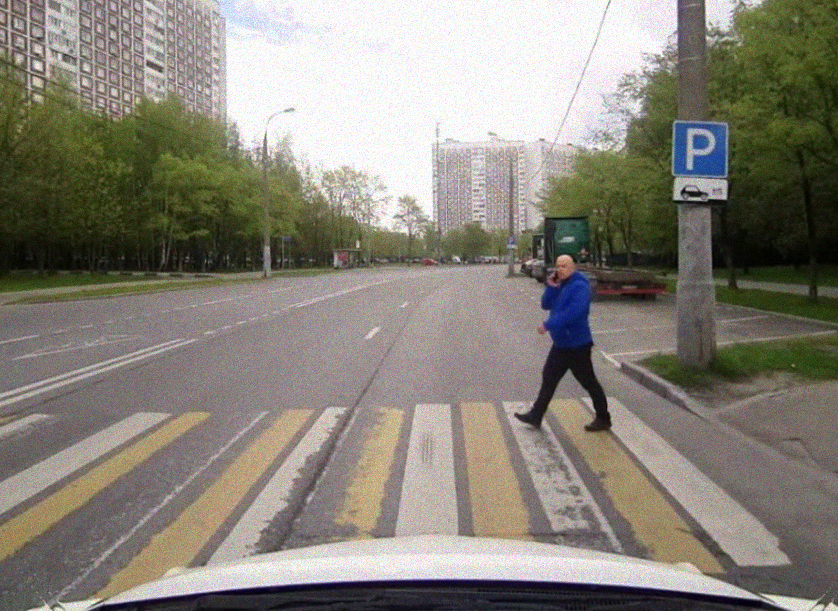
\includegraphics[width=0.6\textwidth]{../outputs/image_quant_noise.png}
    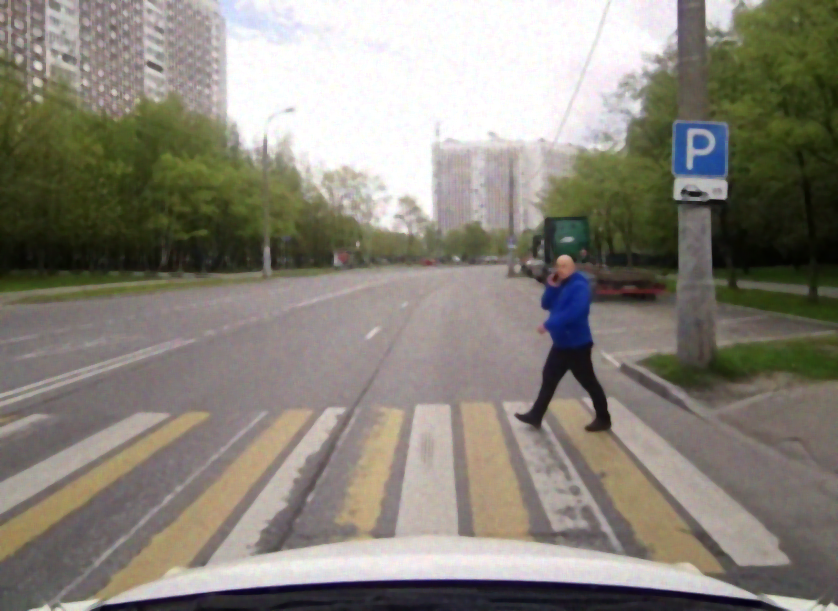
\includegraphics[width=0.6\textwidth]{../addition/image_quant_median_filter_k5.png}
    \caption{Изображение с шумом квантизации до и после применения медианного фильтра}
    \label{fig:stich_images}
\end{figure}

\pagebreak

\subsection{Адаптивная медианная фильтрация}

В данной модификации фильтра скользящее окно
адаптивно увеличивается в зависимости от результата фильтрации.

Основной идеей является увеличение размера окна до тех пор,
пока алгоритм не найдет медианное значение, не являющееся импульсным шумом, или пока 
не достигнет максимального размера окна.

\begin{lstlisting}[style=cpp_white, caption={Функции для применения адаптивного медианного фильтра}]
uchar adaptiveProcess(const cv::Mat &im, int row, int col, int kernelSize, int maxSize)
{
    std::vector <uchar> pixels;
    for(int a = -kernelSize / 2; a <= kernelSize / 2; a++){
        for(int b = -kernelSize / 2; b <= kernelSize / 2; b++){
            pixels.push_back(im.at<uchar>(row + a, col + b));
        }
    }
    std::sort(pixels.begin(), pixels.end());
    auto min = pixels[0];
    auto max = pixels[kernelSize * kernelSize - 1];
    auto med = pixels[kernelSize * kernelSize / 2];
    auto zxy = im.at<uchar>(row, col);
    if(med > min && med < max){
        if(zxy > min && zxy < max){
            return zxy;
        }else{
            return med;
        }
    }
    else{
        kernelSize += 2;
        if(kernelSize <= maxSize)
            return adaptiveProcess(im, row, col, kernelSize, maxSize);
        else
            return med;
    }
}

cv::Mat amf_work(cv::Mat src){
    cv::Mat dst;
    int minSize = 3;
    int maxSize = 7; 
    copyMakeBorder(src, dst, maxSize / 2, maxSize / 2, maxSize / 2, maxSize / 2, cv::BORDER_REFLECT);
    int rows = dst.rows;
    int cols = dst.cols;
    for(int j = maxSize / 2; j < rows - maxSize / 2; j++){
        for(int i = maxSize / 2; i < cols * dst.channels() - maxSize / 2; i++){
            dst.at<uchar>(j, i) = adaptiveProcess(dst, j, i, minSize, maxSize);
        }
    }
    return dst;
}
\end{lstlisting}

Применим к изображению с импульссивным шумом адаптивную медианную фильтрацию:

\begin{figure}[hbt!]
    \centering
    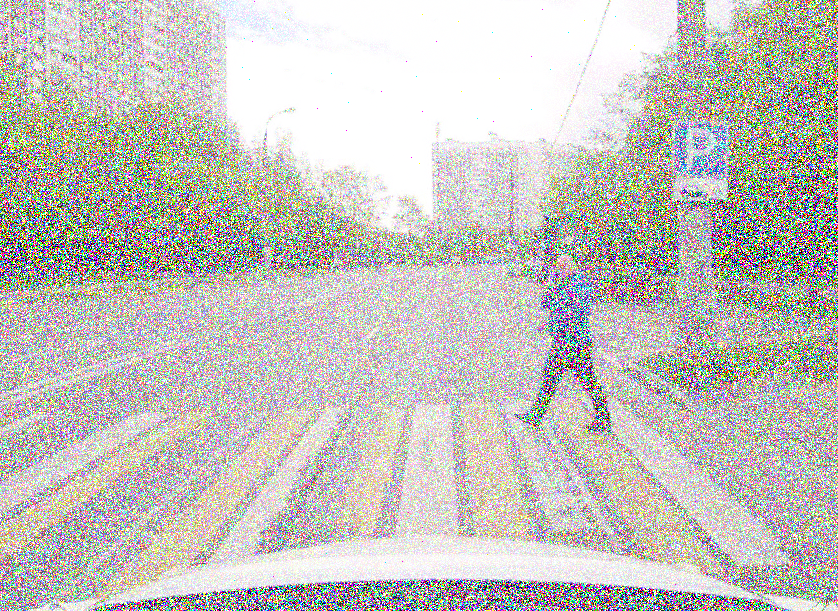
\includegraphics[width=0.6\textwidth]{../outputs/image_impulse_noise.png}
    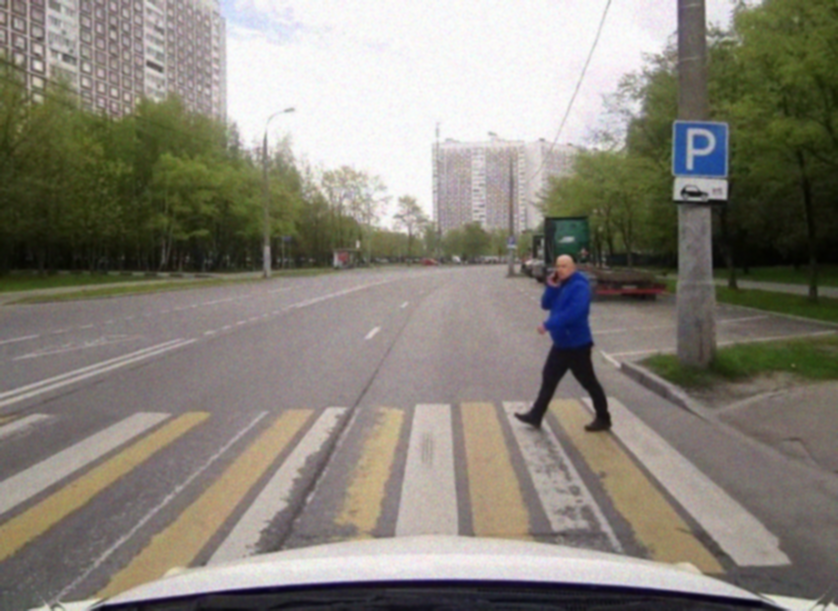
\includegraphics[width=0.6\textwidth]{../outputs/image_quant_filter.png}
    \caption{Изображение с импульсивным шумом до и после применения адаптивного медианного фильтра}
    \label{fig:stich_images}
\end{figure}

\pagebreak
Применим к изображению с мультипликативным шумом адаптивную медианную фильтрацию:

\begin{figure}[hbt!]
    \centering
    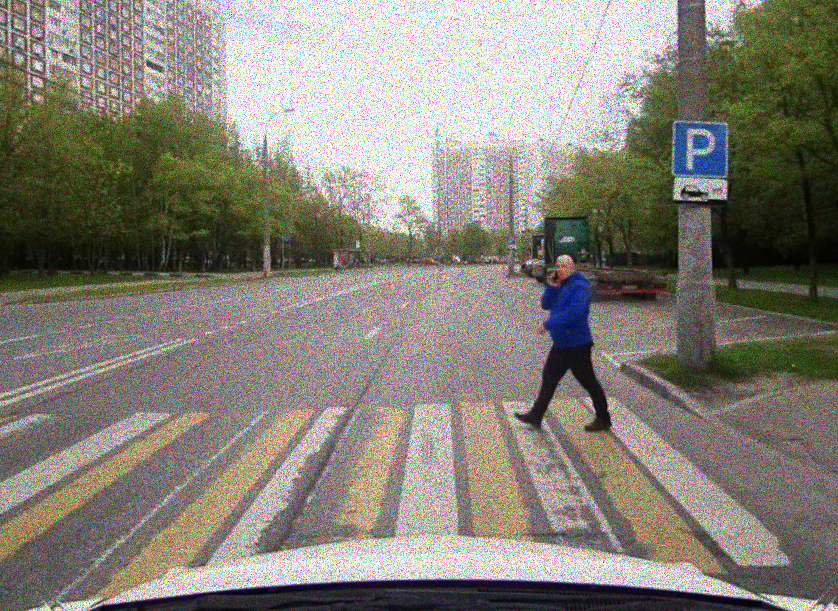
\includegraphics[width=0.6\textwidth]{../outputs/image_mltp_noise.png}
    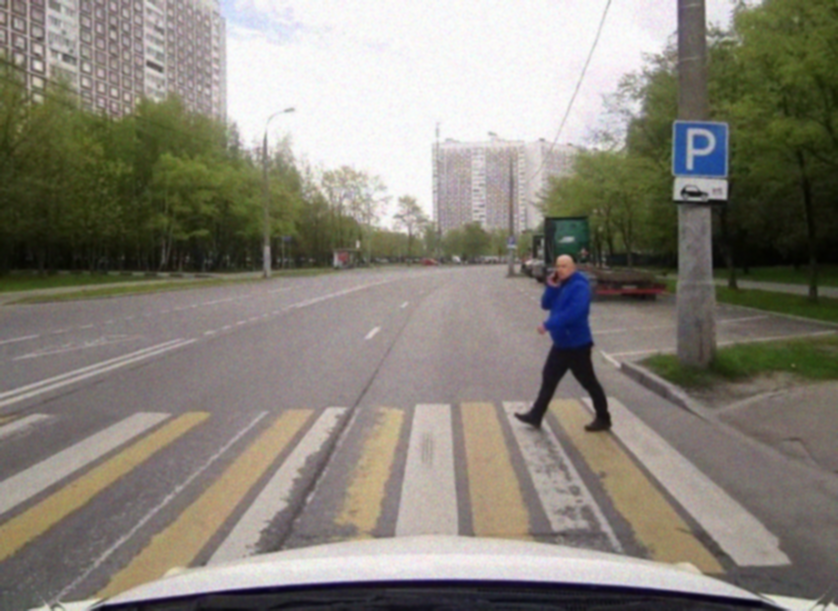
\includegraphics[width=0.6\textwidth]{../outputs/image_quant_filter.png}
    \caption{Изображение с мультипликативным шумом до и после применения адаптивного медианного фильтра}
    \label{fig:stich_images}
\end{figure}

\pagebreak
Применим к изображениям с гауссовским шумом адаптивную медианную фильтрацию:

\begin{figure}[hbt!]
    \centering
    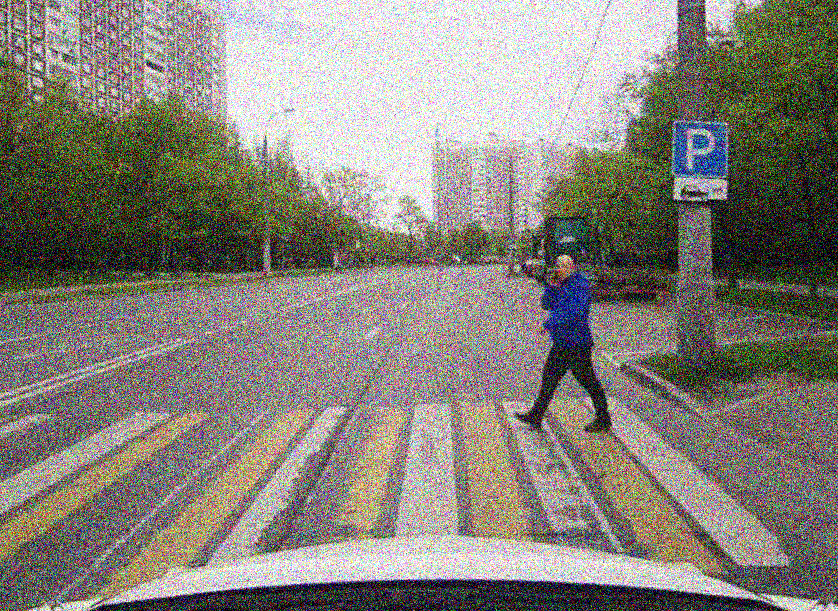
\includegraphics[width=0.6\textwidth]{../outputs/image_gauss_noise.png}
    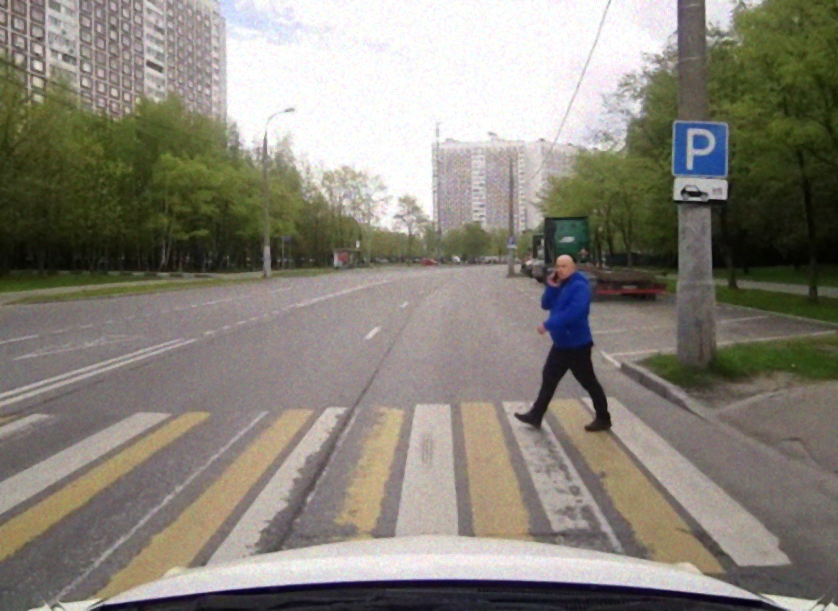
\includegraphics[width=0.6\textwidth]{../addition/image_gauss_quant_filter_k3.png}
    \caption{Изображение с гауссовским шумом до и после применения адаптивного медианного фильтра}
    \label{fig:stich_images}
\end{figure}

\pagebreak
Применим к изображениям с шумом квантизации адаптивную медианную фильтрацию:

\begin{figure}[ht]
    \centering
    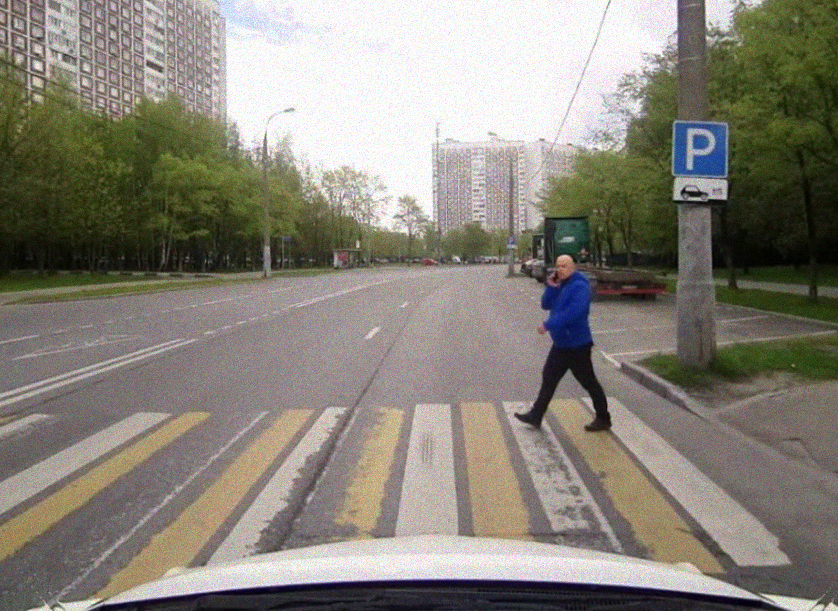
\includegraphics[width=0.6\textwidth]{../outputs/image_quant_noise.png}
    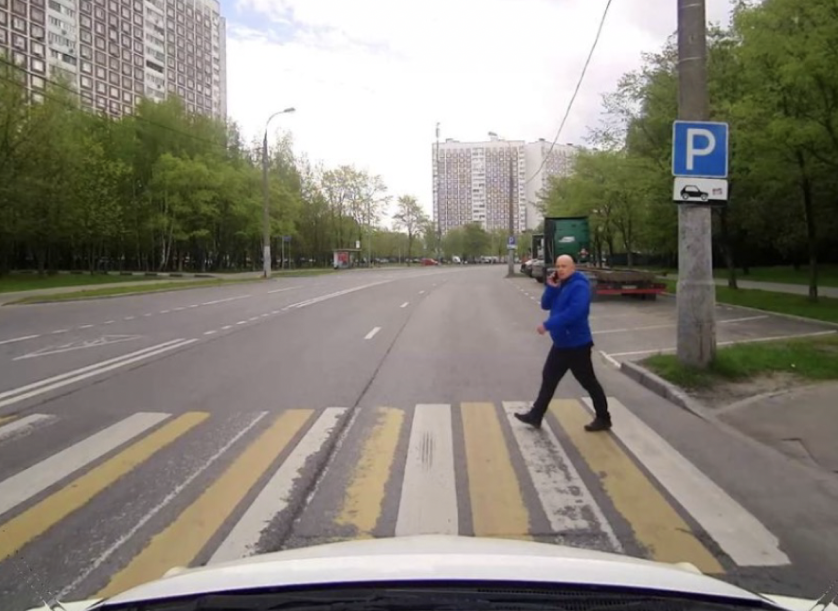
\includegraphics[width=0.6\textwidth]{../source/image.png}
    \caption{Изображение с шумом квантизации до и после применения адаптивного медианного фильтра}
    \label{fig:stich_images}
\end{figure}

\pagebreak

\subsection{Винеровская фильтрация}

Использует пиксельно-адаптивный метод Винера, основанный
на статистических данных, оцененных из локальной окрестности
каждого пикселя.

\begin{lstlisting}[style=cpp_white, caption={Исходный код Винеровского фильтра}]
int k_size[] = {5, 5};
cv::Mat kernel = cv::Mat::ones(k_size[0], k_size[1], CV_64F);

double k_sum = cv::sum(kernel)[0];

cv::Mat image_copy;
if(image.depth() == CV_8U)
    image.convertTo(image_copy, CV_32F, 1.0 / 255);\
else    
    image_copy = image;
cv::copyMakeBorder(image_copy, image_copy,
                    int((k_size[0] - 1) / 2),
                    int(k_size[0] / 2),
                    int((k_size[1] - 1) / 2),
                    int(k_size[1] / 2), cv::BORDER_REPLICATE);

std::vector<cv::Mat> bgr_planes;
cv::split(image_copy, bgr_planes);

for(int k = 0; k < bgr_planes.size(); k++){
    cv::Mat image_tmp = cv::Mat::zeros(image.size(), bgr_planes[k].type());
    double v(0);

    for(int i = 0; i < image.rows; i++)
        for(int j = 0; j < image.cols; j++){
            double m(0), q(0);
            for(int a = 0; a < k_size[0]; a++)
                for(int b = 0; b < k_size[1]; b++){
                    double t = bgr_planes[k].at<float>(i + a, j + b) * kernel.at<double>(a, b);
                    m += t;
                    q += t*t;
                }
            
            m /= k_sum;
            q /= k_sum;
            q -= m*m;
            v += q;
        }
    v /= image.cols * image.rows;

    for(int i = 0; i < image.rows; i++)
        for(int j = 0; j < image.cols; j++){
            double m(0), q(0);
            for(int a = 0; a < k_size[0]; a++)
                for(int b = 0; b < k_size[1]; b++){
                    double t = bgr_planes[k].at<float>(i = a, j + b) * kernel.at<double>(a, b);
                    m += t;
                    q += t*t;
                }
            m /= k_sum;
            q /= k_sum;
            q -= m*m;

            double im = bgr_planes[k].at<float>(i + (k_size[0] - 1) / 2, j + (k_size[1] - 1) / 2);
            if(q < v)
                image_tmp.at<float>(i, j) = float(m);
            else
                image.at<float>(i, j) = float((im - m) * ( 1 - v / q) + m);
        }
    bgr_planes[k] = image_tmp;
}

cv::merge(bgr_planes, image_out);
\end{lstlisting}

Применим к изображению с импульссивным шумом Винеровскую фильтрацию:

\begin{figure}[hbt!]
    \centering
    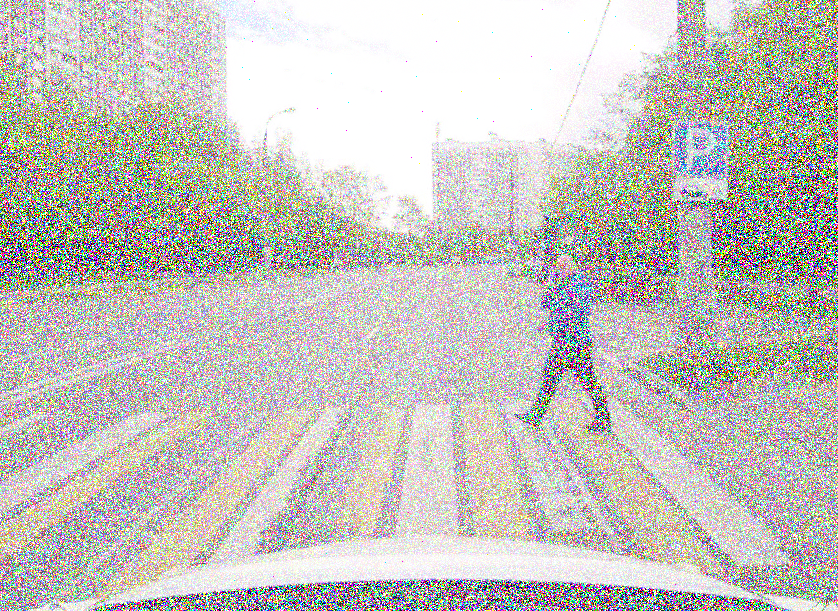
\includegraphics[width=0.6\textwidth]{../outputs/image_impulse_noise.png}
    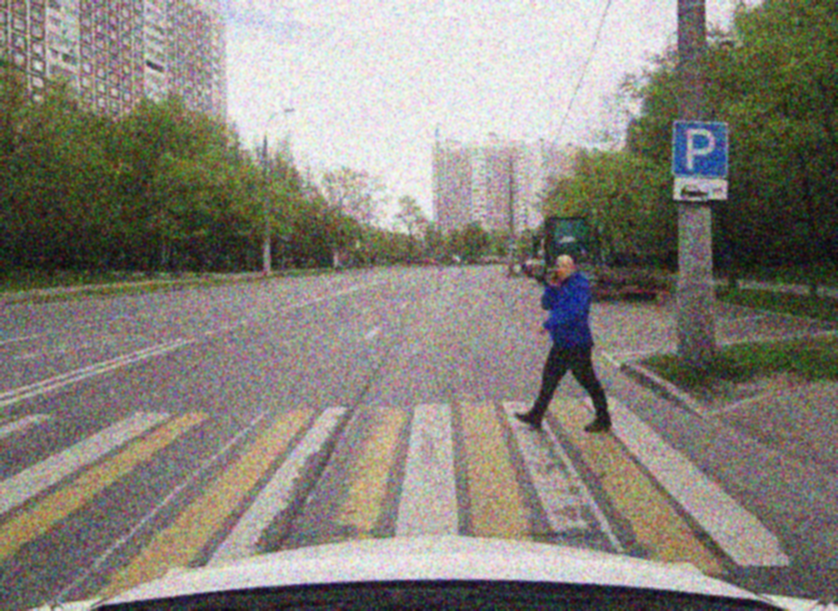
\includegraphics[width=0.6\textwidth]{../outputs/image_gaussian_filter.png}
    \caption{Изображение с импульсивным шумом до и после применения Винеровской фильтрации}
    \label{fig:stich_images}
\end{figure}

\pagebreak
Применим к изображению с мультипликативным шумом Винеровскую фильтрацию:

\begin{figure}[hbt!]
    \centering
    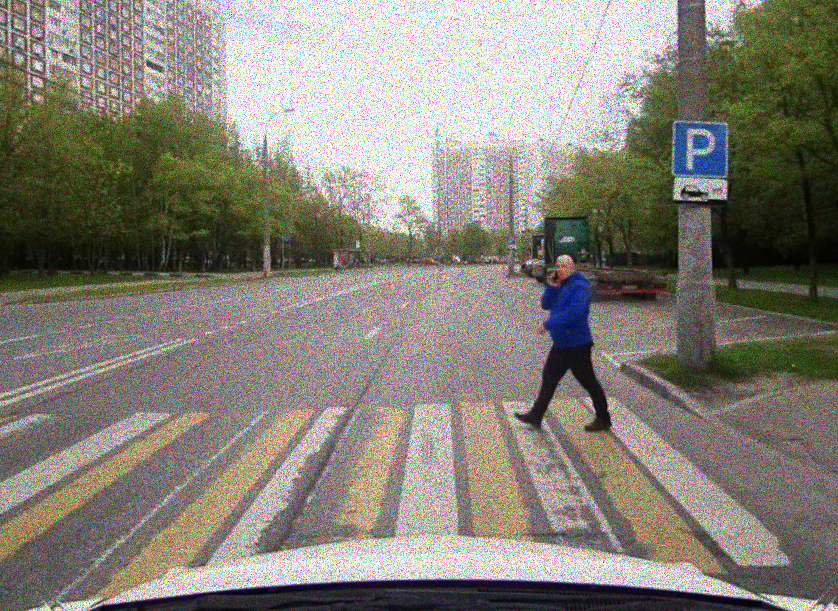
\includegraphics[width=0.6\textwidth]{../outputs/image_mltp_noise.png}
    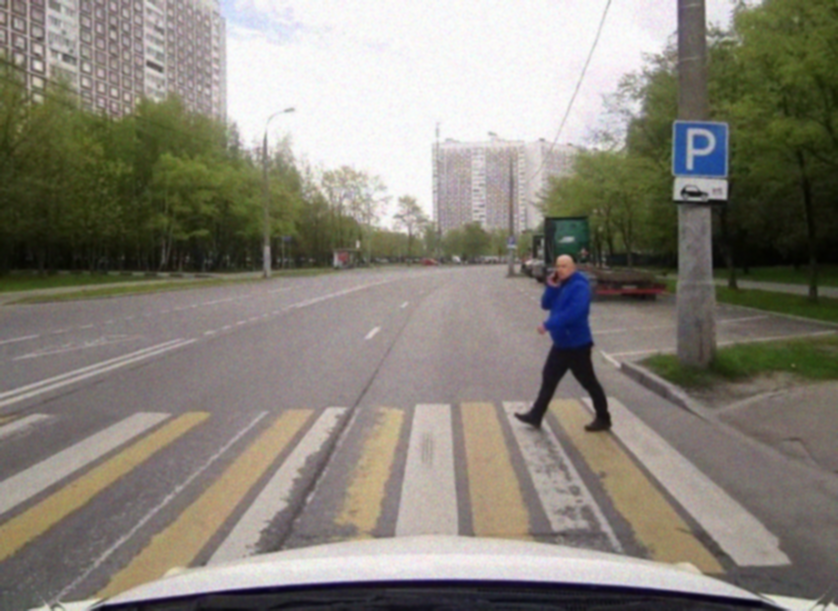
\includegraphics[width=0.6\textwidth]{../outputs/image_quant_filter.png}
    \caption{Изображение с мультипликативным шумом до и после применения Винеровской фильтрации}
    \label{fig:stich_images}
\end{figure}

\pagebreak
Применим к изображениям с гауссовским шумом Винеровскую фильтрацию:

\begin{figure}[hbt!]
    \centering
    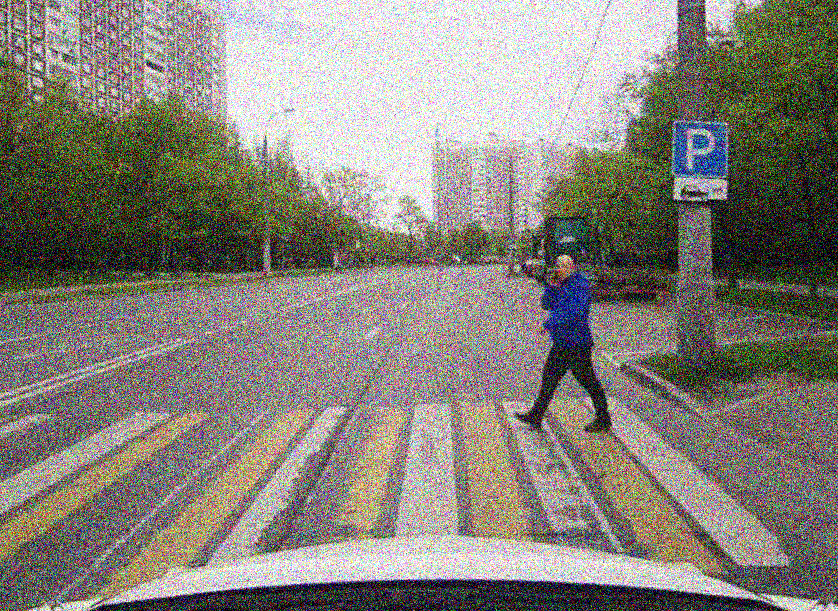
\includegraphics[width=0.6\textwidth]{../outputs/image_gauss_noise.png}
    \includegraphics[width=0.6\textwidth]{../addition/image_gauss_quant_filter_k3.png}
    \caption{Изображение с гауссовским шумом до и после применения Винеровской фильтрации}
    \label{fig:stich_images}
\end{figure}

\pagebreak
Применим к изображениям с шумом квантизации Винеровскую фильтрацию:

\begin{figure}[ht]
    \centering
    \includegraphics[width=0.6\textwidth]{../outputs/image_quant_noise.png}
    \includegraphics[width=0.6\textwidth]{../source/image.png}
    \caption{Изображение с шумом квантизации до и после применения Винеровской фильтрации}
    \label{fig:stich_images}
\end{figure}

\pagebreak

\section{Высокочастотная фильтрация}

\begin{figure}[ht]
    \centering
    \includegraphics[width=\textwidth]{../source/SDC_Yandex.png}
    \caption{Исходное изображение}
    \label{fig:stitch_images}
\end{figure}



\subsection{Фильтр Робертса}

Фильтр Робертса работает с минимально допустимой для вычисления производной маской размерности 
2×2, поэтому является быстрым и довольно эффективным. Возможные варианты масок
для нахождения градиента по осям $Ox$ и $Oy$:

\begin{equation}
    G_x = \begin{bmatrix}
        1 & 0 \\
        0 & 1 
    \end{bmatrix}, 
    G_y = \begin{bmatrix}
        1 & 0 \\
        -1 & 0 
    \end{bmatrix}
\end{equation}

\begin{lstlisting}[style=cpp_white, caption={Исходный код фильтра Робертса}]
cv::Mat G_x = (cv::Mat_<double>(2, 2) << -1, 1, 0, 0);
cv::Mat G_y = (cv::Mat_<double>(2, 2) << 1, 0, -1, 0);

cv::Mat I_x, I_y, I_out;

cv::filter2D(image, I_x, -1, G_x);
cv::filter2D(image, I_y, -1, G_y);

I_x.convertTo(I_x, CV_32F);
I_y.convertTo(I_y, CV_32F);

cv::magnitude(I_x, I_y, I_out);
\end{lstlisting}

\begin{figure}[ht]
    \centering
    \includegraphics[width=\textwidth]{../outputs/roberts_operator.png}
    \caption{Изображение после применения фильтра Робертса}
    \label{fig:stitch_images}
\end{figure}

\pagebreak

\subsection{Фильтр Превитта}

В данном подходе используются две ортогональные маски размером 3 × 3, позволяющие более точно вычислить производные по
осям $Ox$ и $Oy$:

\begin{equation}
    G_x = \begin{bmatrix}
        -1 & 0 & 1 \\
        -1 & 0 & 1 \\
        -1 & 0 & 1
    \end{bmatrix}, 
    G_y = \begin{bmatrix}
        -1 & -1 & -1 \\
        0 & 0 & 0 \\
        1 & 1 & 1
    \end{bmatrix}
\end{equation}

\begin{lstlisting}[style=cpp_white, caption={Исходный код фильтра Превитта}]
image = cv::imread(path + "/lab3/source/SDC_Yandex.png", 1);
cv::Mat G_x = (cv::Mat_<double>(3, 3) << -1, 0, 1, -1, 0, 1, -1, 0, 1);
cv::Mat G_y = (cv::Mat_<double>(3, 3) << -1, -1, -1, 0, 0, 0, 1, 1, 1);

cv::Mat I_x, I_y, I_out;

cv::filter2D(image, I_x, -1, G_x);
cv::filter2D(image, I_y, -1, G_y);

I_x.convertTo(I_x, CV_32F);
I_y.convertTo(I_y, CV_32F);

cv::magnitude(I_x, I_y, I_out);
\end{lstlisting}

\begin{figure}[ht]
    \centering
    \includegraphics[width=\textwidth]{../outputs/previt_operator.png}
    \caption{Изображение после применения фильтра Превитта}
    \label{fig:stitch_images}
\end{figure}

\pagebreak

\subsection{Фильтр Превитта}

Данный подход аналогичен фильтру Робертса, однако используются разные веса в масках. 
Типичный пример фильтра Собела:

\begin{equation}
    G_x = \begin{bmatrix}
        -1 & 0 & 1 \\
        -2 & 0 & 2 \\
        -1 & 0 & 1
    \end{bmatrix}, 
    G_y = \begin{bmatrix}
        -1 & -2 & -1 \\
        0 & 0 & 0 \\
        1 & 2 & 1
    \end{bmatrix}
\end{equation}

\begin{lstlisting}[style=cpp_white, caption={Исходный код фильтра Собела}]
image = cv::imread(path + "/lab3/source/SDC_Yandex.png", 1);
cv::Mat G_x = (cv::Mat_<double>(3, 3) << -1, 0, 1, -2, 0, 2, -1, 0, 1);
cv::Mat G_y = (cv::Mat_<double>(3, 3) << 1, 2, 1, 0, 0, 0, -1, -2, -1);

cv::Mat I_x, I_y, I_out;

cv::filter2D(image, I_x, -1, G_x);
cv::filter2D(image, I_y, -1, G_y);

I_x.convertTo(I_x, CV_32F);
I_y.convertTo(I_y, CV_32F);

cv::magnitude(I_x, I_y, I_out);
\end{lstlisting}

\begin{figure}[ht]
    \centering
    \includegraphics[width=\textwidth]{../outputs/sobel_operator.png}
    \caption{Изображение после применения фильтра Собела}
    \label{fig:stitch_images}
\end{figure}

\pagebreak

\subsection{Фильтр Лапласа}

Фильтр Лапласа использует аппроксимацию вторых производ-
ных по осям $Ox$ и $Oy$, в отличие от предыдущих подходов, исполь-
зующих первую производную. Формула:

\begin{equation}
    w = \begin{bmatrix}
        0 & -1 & 0 \\
        -1 & 4 & -1 \\
        0 & -1 & 0
    \end{bmatrix}
\end{equation}

\begin{lstlisting}[style=cpp_white, caption={Исходный код фильтра Лапласа}]
image = cv::imread(path + "/lab3/source/SDC_Yandex.png", 1);
cv::Mat G_x = (cv::Mat_<double>(3, 3) << 0, -1, 0, -1, 4, -1, 0, -1, 0);
cv::Mat G_y = (cv::Mat_<double>(3, 3) << 0, -1, 0, -1, 4, -1, 0, -1, 0);

cv::Mat I_x, I_y, I_out;

cv::filter2D(image, I_x, -1, G_x);
cv::filter2D(image, I_y, -1, G_y);

I_x.convertTo(I_x, CV_32F);
I_y.convertTo(I_y, CV_32F);

cv::magnitude(I_x, I_y, I_out);
\end{lstlisting}

\begin{figure}[ht]
    \centering
    \includegraphics[width=\textwidth]{../outputs/laplas_operator.png}
    \caption{Изображение после применения фильтра Лапласа}
    \label{fig:stitch_images}
\end{figure}

\pagebreak

\subsection{Алгоритм Кэнни}

Одним из самых распространенных и эффективных алгоритмов
выделения контуров на изображении является алгоритм Кэнни.
Данный алгоритм позволяет не только определять краевые пиксе-
ли, но и связные граничные линии.

\begin{lstlisting}[style=cpp_white, caption={Исходный код применения алгоритма Кэнни}]
image = cv::imread(path + "/lab3/source/SDC_Yandex.png", 1);
cv::Canny(image, image_out, 50, 200);
\end{lstlisting}

\begin{figure}[ht]
    \centering
    \includegraphics[width=\textwidth]{../outputs/canny_operator.png}
    \caption{Изображение после применения алгоритма Кэнни}
    \label{fig:stitch_images}
\end{figure}

\pagebreak

\section{Выводы}
В процессе выполнения лабораторной работы мы освоили основные виды фильтраций изображений и использовали различные алгоритмы выделения границ на озображении, попробовали скорректировать шумы. 

Также смогли оценить качество полученных изображений и убедиться, что фильтрация позволяет улучшать их визуальное восприятие

\section{Ответы на вопросы}

\newcounter{question}
\setcounter{question}{0}

\newcommand{\question}[1]{\item[Q\refstepcounter{question}\thequestion.] #1}
\newcommand{\answer}[1]{\item[A\thequestion.] #1}

\begin{itemize}

\question{В чем заключаются основные недостатки адаптивных методов фильтрации изображений?}
\answer{Основными минусами данного метода являются: сильное размытие рисунка при недостаточном контрасте между светлыми и темными участками изображения и чувствительность к импульсивным помехам, Возможность возникновения артефактов: в некоторых случаях адаптивные методы фильтрации могут приводить к появлению артефактов на изображениях, таких как размытие границ объектов или искажение текстур, Вычислительная сложность: адаптивные методы фильтрации могут быть более ресурсоемкими по сравнению с классическими методами, так как они требуют выполнения дополнительных вычислений для определения параметров фильтра.}

\question{При каких значениях параметра $Q$ контргармонический
фильтр будет работать как арифметический, а при каких как гармонический?}
\answer{При $Q$ = 0 фильтр превращается в арифметический, а при $Q$ = -1 — в гармонический.}

\question{Какими операторами можно выделить границы на изображении?}
\answer{На изображении можно выделить границы с помощью операторов, таких как оператор Собеля, оператор Робертса, оператор Превитта, оператор Кэнни, оператор Лапласа и т.д.}

\question{Для чего на первом шаге выделения контуров, как правило,
выполняется низкочастотная фильтрация?}
\answer{Низкочастотная фильтрация на первом шаге выделения контуров используется для сглаживания изображения и уменьшения шумов, которые могут помешать правильному определению контуров. Фильтрация помогает убрать мелкие детали и делает контуры более четкими и выраженными, что облегчает дальнейший процесс обработки изображения.}

\end{itemize}

